%----------------------------------------------------------------------------------------
%	PACKAGES AND THEMES
%----------------------------------------------------------------------------------------

\documentclass[10pt]{beamer}

\mode<presentation> {

% The Beamer class comes with a number of default slide themes
% which change the colors and layouts of slides. Below this is a list
% of all the themes, uncomment each in turn to see what they look like.

%\usetheme{default}
%\usetheme{AnnArbor}
%\usetheme{Antibes}
%\usetheme{Bergen}
%\usetheme{Berkeley}
%\usetheme{Berlin}
%\usetheme{Boadilla}
%\usetheme{CambridgeUS}
%\usetheme{Copenhagen}
%\usetheme{Darmstadt}
%\usetheme{Dresden}
%\usetheme{Frankfurt}
%\usetheme{Goettingen}
%\usetheme{Hannover}
%\usetheme{Ilmenau}
%\usetheme{JuanLesPins}
%\usetheme{Luebeck}
\usetheme{Madrid}
%\usetheme{Malmoe}
%\usetheme{Marburg}
%\usetheme{Montpellier}
%\usetheme{PaloAlto}
%\usetheme{Pittsburgh}
%\usetheme{Rochester}
%\usetheme{Singapore}
%\usetheme{Szeged}
%\usetheme{Warsaw}

% As well as themes, the Beamer class has a number of color themes
% for any slide theme. Uncomment each of these in turn to see how it
% changes the colors of your current slide theme.

%\usecolortheme{albatross}
%\usecolortheme{beaver}
%\usecolortheme{beetle}
%\usecolortheme{crane}
%\usecolortheme{dolphin}
%\usecolortheme{dove}
%\usecolortheme{fly}
%\usecolortheme{lily}
%\usecolortheme{orchid}
%\usecolortheme{rose}
%\usecolortheme{seagull}
%\usecolortheme{seahorse}
%\usecolortheme{whale}
%\usecolortheme{wolverine}

%\setbeamertemplate{footline} % To remove the footer line in all slides uncomment this line
%\setbeamertemplate{footline}[page number] % To replace the footer line in all slides with a simple slide count uncomment this line

\setbeamertemplate{navigation symbols}{} % To remove the navigation symbols from the bottom of all slides uncomment this line
}

\usepackage{graphicx} % Allows including images
\usepackage{booktabs} % Allows the use of \toprule, \midrule and \bottomrule in tables
\usepackage{hyperref}
\usepackage{tikz}
\usepackage{algpseudocode}
\usepackage{algorithm}
\usepackage[makeroom]{cancel}
\usepackage{multicol}
\usepackage{bm}
\setbeamerfont{frametitle}{size=\large}
\setbeamerfont{framesubtitle}{size=\small}
\setbeamertemplate{caption}[numbered]
\usepackage{appendixnumberbeamer}

%----------------------------------------------------------------------------------------
%	TITLE PAGE
%----------------------------------------------------------------------------------------

\title[EMMA]{Energy-based Multi-Modal Attention} % The short title appears at the bottom of every slide, the full title is only on the title page
\subtitle{EMMA}
\author[Aurélien Werenne]{Aurélien Werenne \\ {\small Supervisor: Dr. Raphaël Marée}} 
\institute[ULiège] 
{
\begin{figure}

\includegraphics[scale=0.3]{figs/logo-uliege}
\end{figure}
\medskip
}
\date{September 10, 2019} 

\begin{document}

\begin{frame}
\titlepage 
\end{frame}

%------------------------------------------------
\begin{frame}
\frametitle{Problem \& Solution}
\begin{figure}
\centering
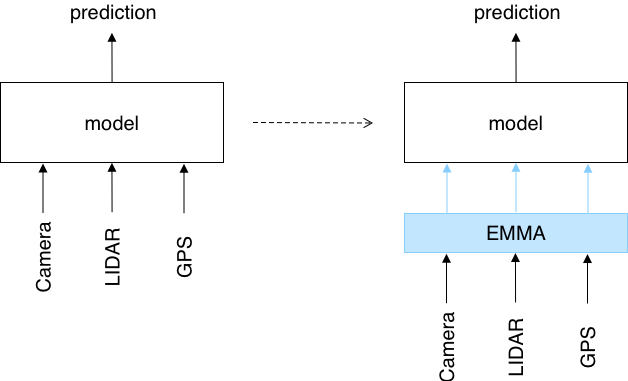
\includegraphics[scale=0.45]{figs/introduction-three-modes-with-emma}
\end{figure}
\end{frame}

%------------------------------------------------
\begin{frame}
\frametitle{Attention scores}
\uncover<1-4>{Module learns how to compute attention scores based on the three properties,}\vspace*{0.25cm}
\begin{itemize}
\uncover<2-4>{\item Relevance: intrinsic informativeness for the predictive task at hand.} \vspace*{0.25cm}

\uncover<3-4>{\item Failure intensity: the propensity to trigger undesirable activations in the neural network.} \vspace*{0.25cm}

\uncover<4-4>{\item Coupling: the interdependencies with the other modes.} \vspace*{0.25cm}
\end{itemize}
\end{frame}



%------------------------------------------------
\begin{frame}
\frametitle{Regularization}
\textbf{Generalize robustness} by using\vspace*{0.25cm}
\begin{itemize}
\item Capacity regularizer: minimize total amount of distributed attention. \vspace*{0.25cm}
\item Energy regularizer: maximize influence of failure intensity.\vspace*{0.25cm}
\end{itemize}
\end{frame}

%------------------------------------------------
\begin{frame}
\frametitle{Result}
\centering
\begin{tabular}{@{}rrrrcrrr@{}}\toprule
& \multicolumn{3}{c}{Hyperparameters} & \phantom{abc}& \multicolumn{3}{c}{F1-score}\\
\cmidrule{2-4} \cmidrule{6-8}
& \multicolumn{1}{c}{$\rho$} & \multicolumn{1}{c}{$\lambda_e$} & \multicolumn{1}{c}{$\lambda_c$} && \multicolumn{1}{r}{uncorrupted} & \multicolumn{1}{r}{IP noisy} & \multicolumn{1}{r}{DM noisy}\\ \midrule\midrule
IP-only & & & && 0.8235 & 0.5926 & \\
DM-only & & & && 0.6612 &  & 0.3920\\\midrule
base & & & && 0.8830 & 0.6441 & 0.6569\\
without & & & && 0.8671& 0.7097& 0.7683\\
other & & & && 0.7726 & 0.6129 & 0.6882\\\midrule
with & $10^{-4}$ & $10^{-3}$ & $10^{-2}$ && $\mathbf{0.8881}$& $\mathbf{0.7333}$& $\mathbf{0.8077}$\\
with & $10^{-4}$ & $0$ & $10^{-2}$ && $\mathbf{0.8849}$& $\mathbf{0.7285}$& $\mathbf{0.8183}$\\
with & $10^{-4}$ & $10^{-4}$ & $10^{-2}$ && $\mathbf{0.8945}$& $\mathbf{0.7333}$& $\mathbf{0.8182}$\\
with & $10^{-3}$ & $10^{-3}$ & $0$ && 0.8809& $\mathbf{0.7347}$& $\mathbf{0.8186}$\\
with & $10^{-4}$ & $10^{-2}$ & $10^{-3}$ && 0.8736& $\mathbf{0.7383}$& $\mathbf{0.7848}$\\
with & $10^{-1}$ & $10^{-2}$ & $0$ && 0.8826& $\mathbf{0.7467}$& $\mathbf{0.7925}$\\
with & $10^{-4}$ & $10^{-3}$ & $0$ && 0.8786& $\mathbf{0.7190}$& $\mathbf{0.7826}$\\
with & $10^{-3}$ & $10^{-1}$ & $10^{-2}$ && 0.8800& $\mathbf{0.7432}$& $\mathbf{0.8344}$\\
with & $10^{-4}$ & $0$ & $10^{-4}$ && 0.8723& 0.7051& $\mathbf{0.7853}$\\
with & $10^{-4}$ & $10^{-4}$ & $10^{-3}$ && 0.8794& 0.7053& $\mathbf{0.7853}$\\
\bottomrule
\end{tabular}
\end{frame}

%------------------------------------------------
\begin{frame}
\frametitle{Robustness generalization}
\begin{multicols}{2}
\begin{figure}
\centering
\begin{overprint}
    \onslide<1>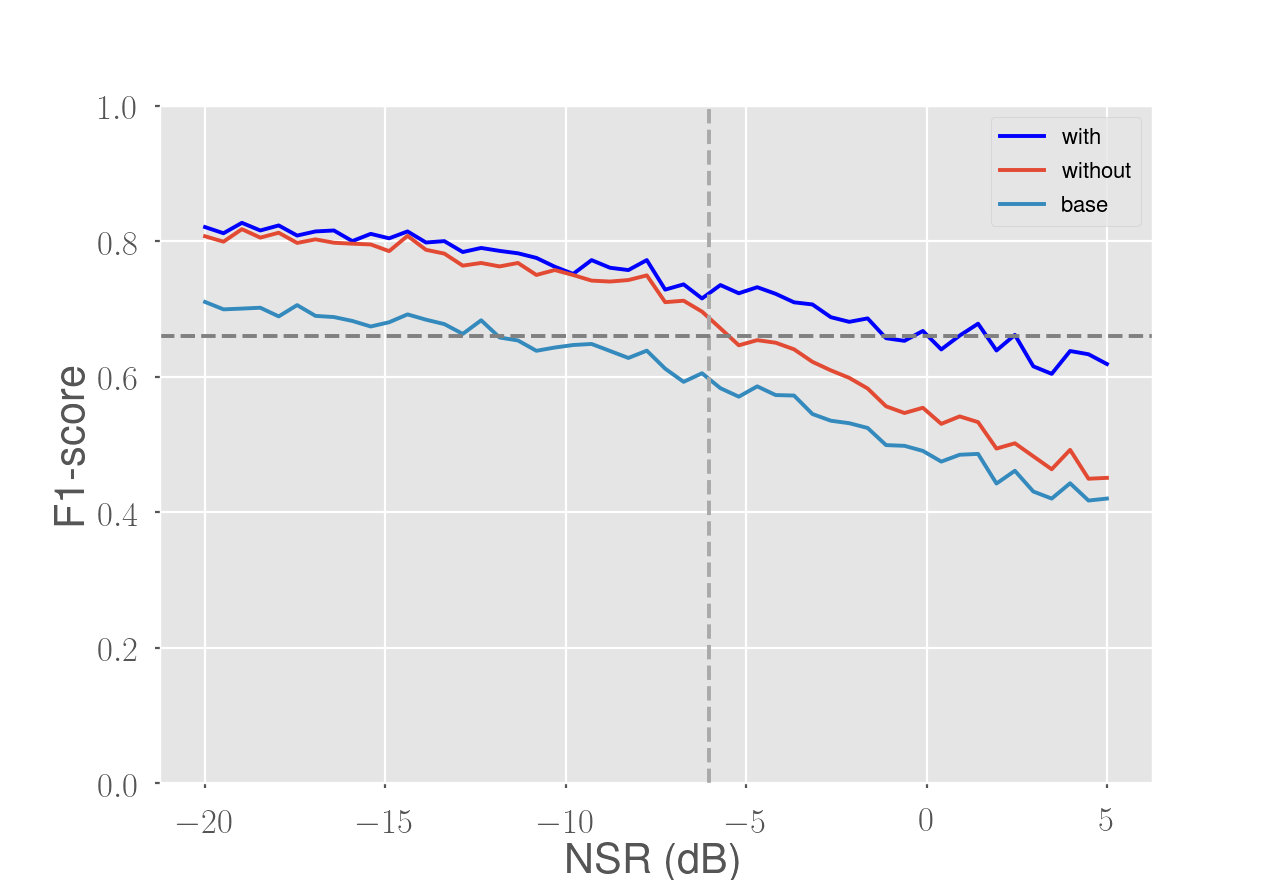
\includegraphics[scale=0.2]{figs/noise-generalisation-ip-noisy}
\end{overprint}
\caption{F1-score, noisy IP-mode}
\end{figure}
\columnbreak
\begin{figure}
\centering
\begin{overprint}
    \onslide<1>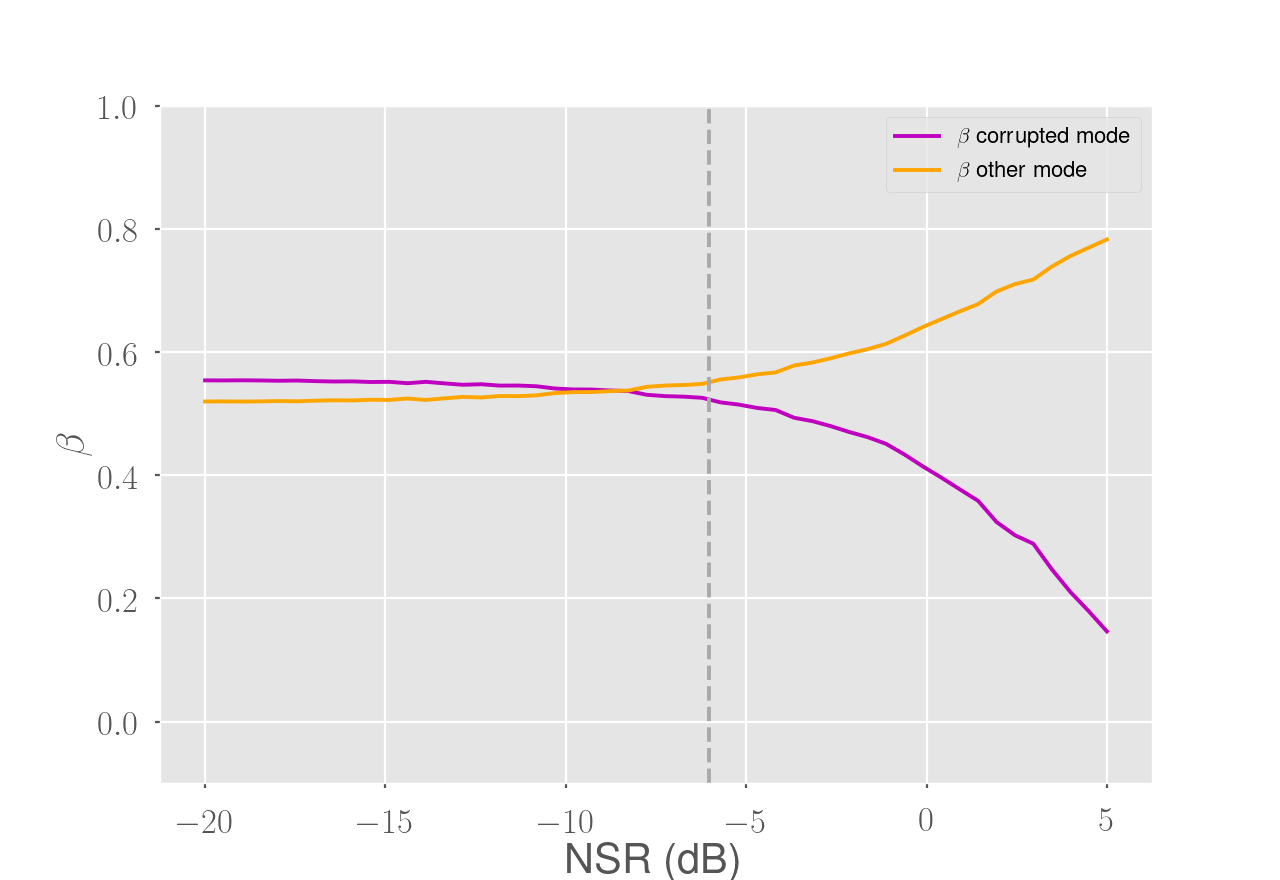
\includegraphics[scale=0.2]{figs/normal-ip-noisy-beta}
\end{overprint}
\caption{attention score, noisy IP-mode}
\end{figure}
\end{multicols}
\end{frame}

%------------------------------------------------
\begin{frame}
\frametitle{Robustness generalization for DM mode}
\begin{multicols}{2}
\begin{figure}
\centering
\begin{overprint}
    \onslide<1>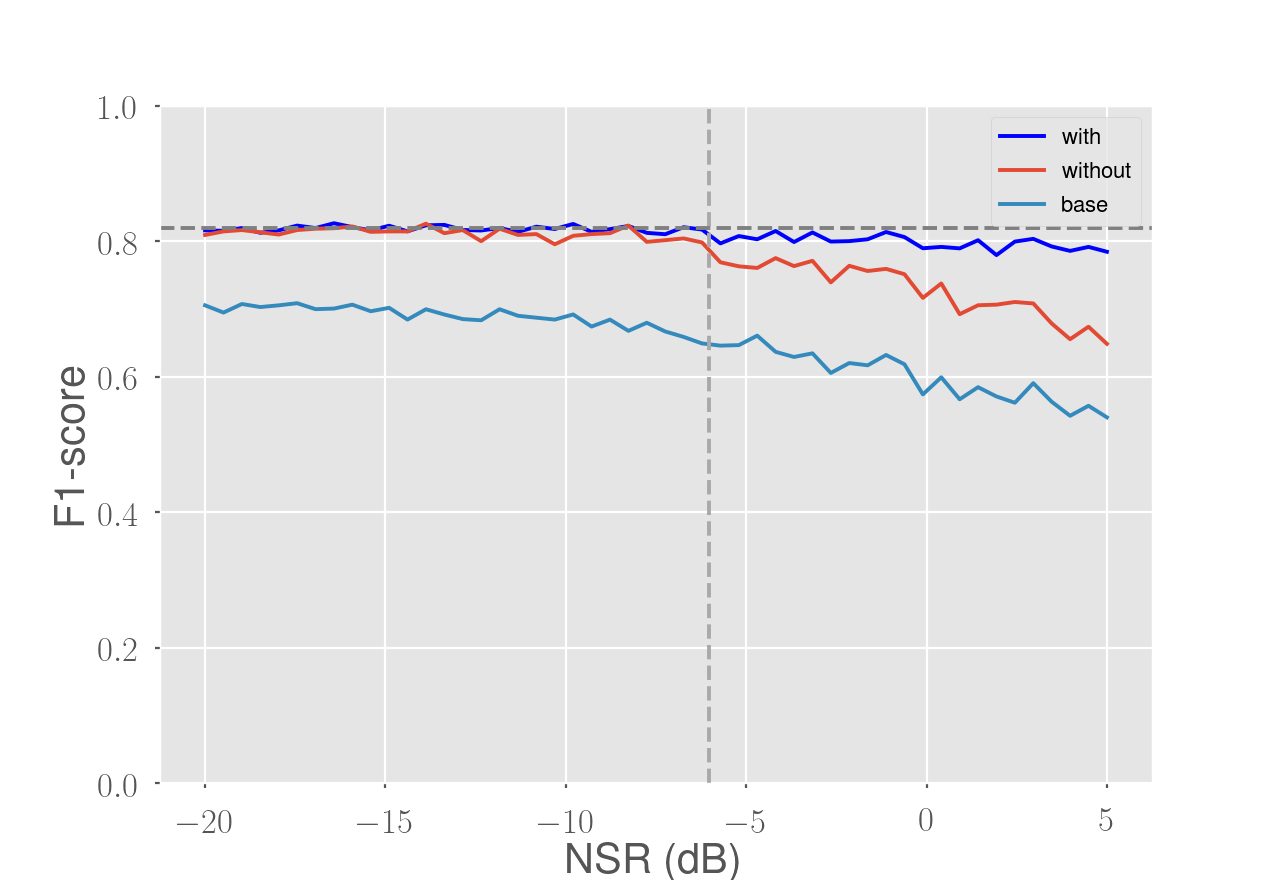
\includegraphics[scale=0.2]{figs/noise-generalisation-dm-noisy}
\end{overprint}
\caption{F1-score, noisy DM-mode}
\end{figure}
\columnbreak
\begin{figure}
\centering
\begin{overprint}
    \onslide<1>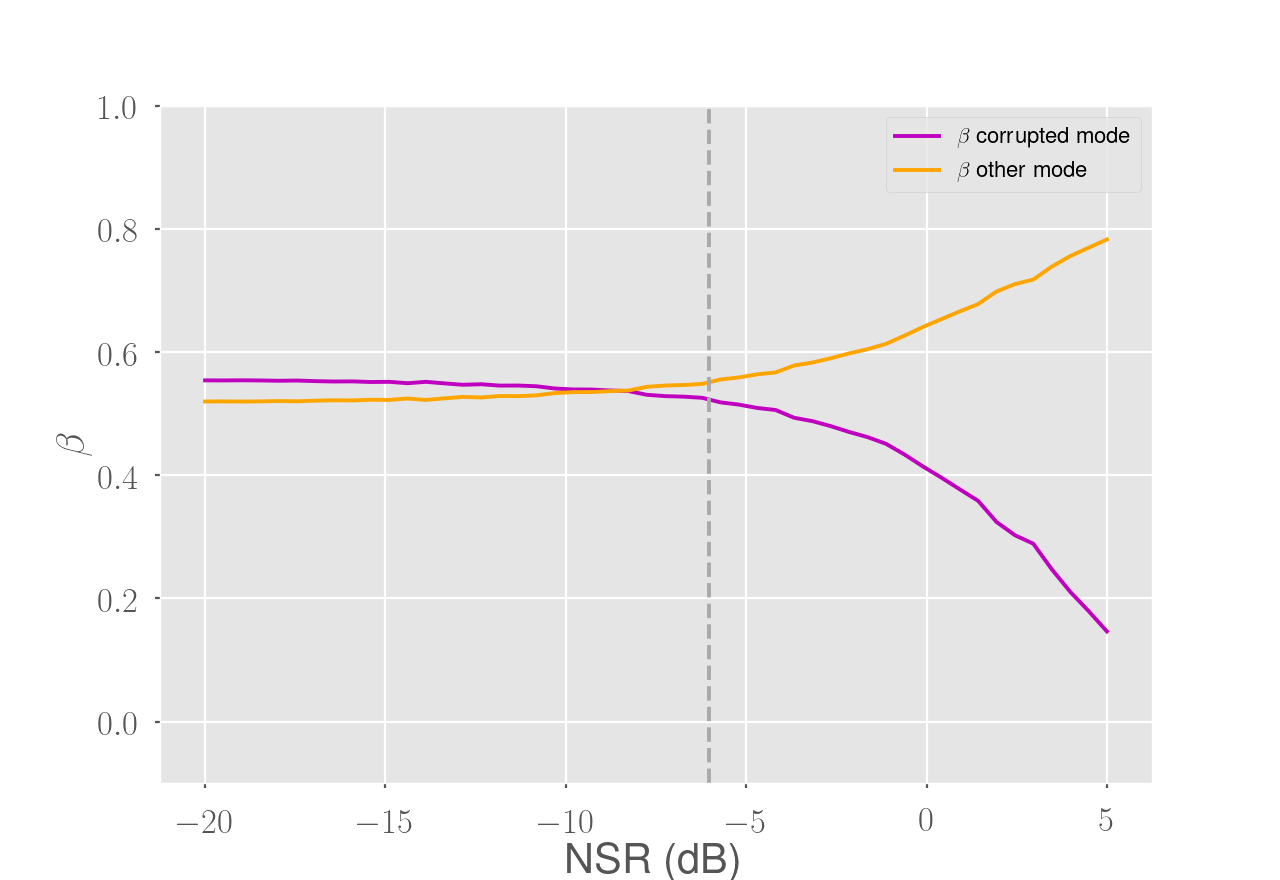
\includegraphics[scale=0.2]{figs/normal-ip-noisy-beta}
\end{overprint}
\caption{attention score, noisy DM-mode}
\end{figure}
\end{multicols}
\end{frame}

%------------------------------------------------
\begin{frame}
\frametitle{Influence of capacity minimization}
\begin{multicols}{2}
\begin{figure}
\centering
\begin{overprint}
    \onslide<1>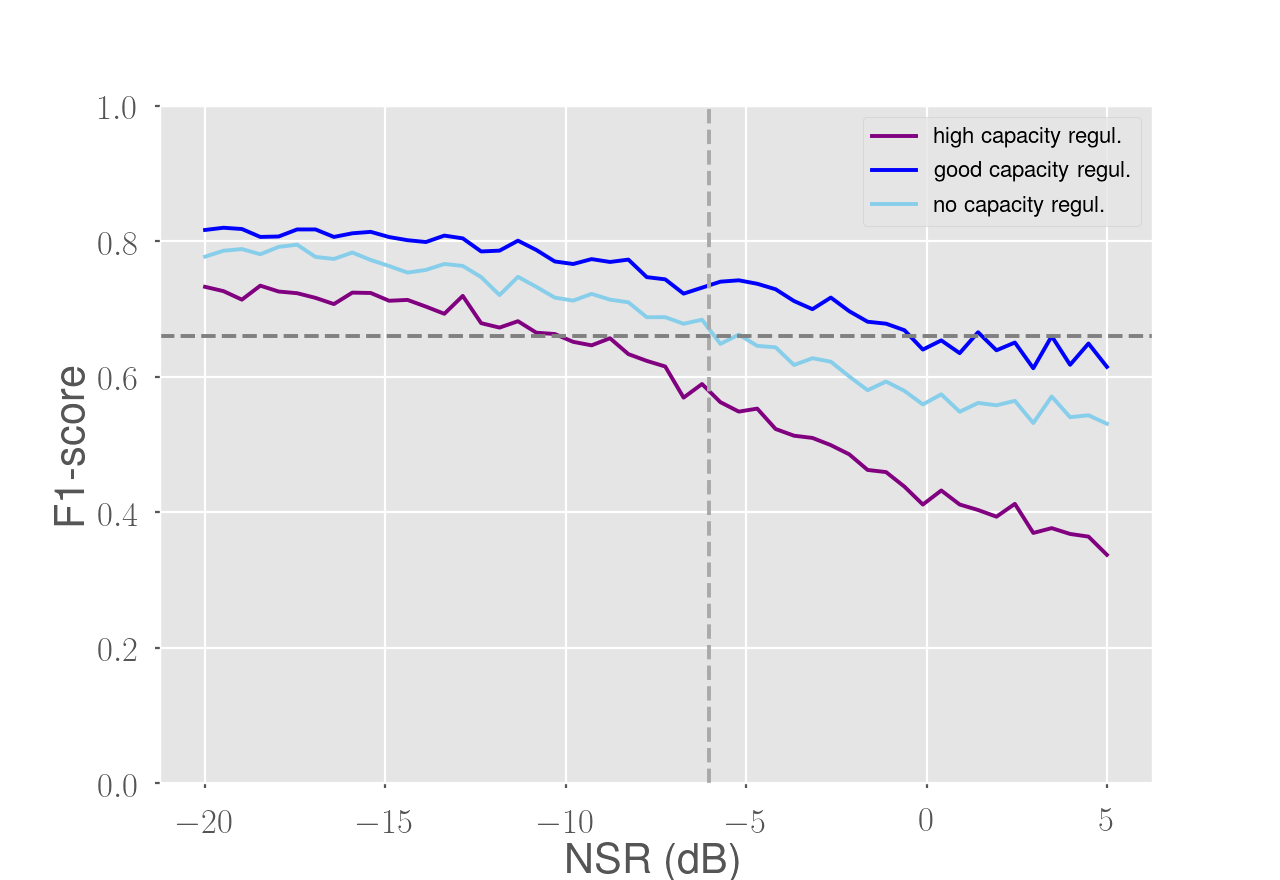
\includegraphics[scale=0.2]{figs/capacity-ip-noisy}
    \onslide<2>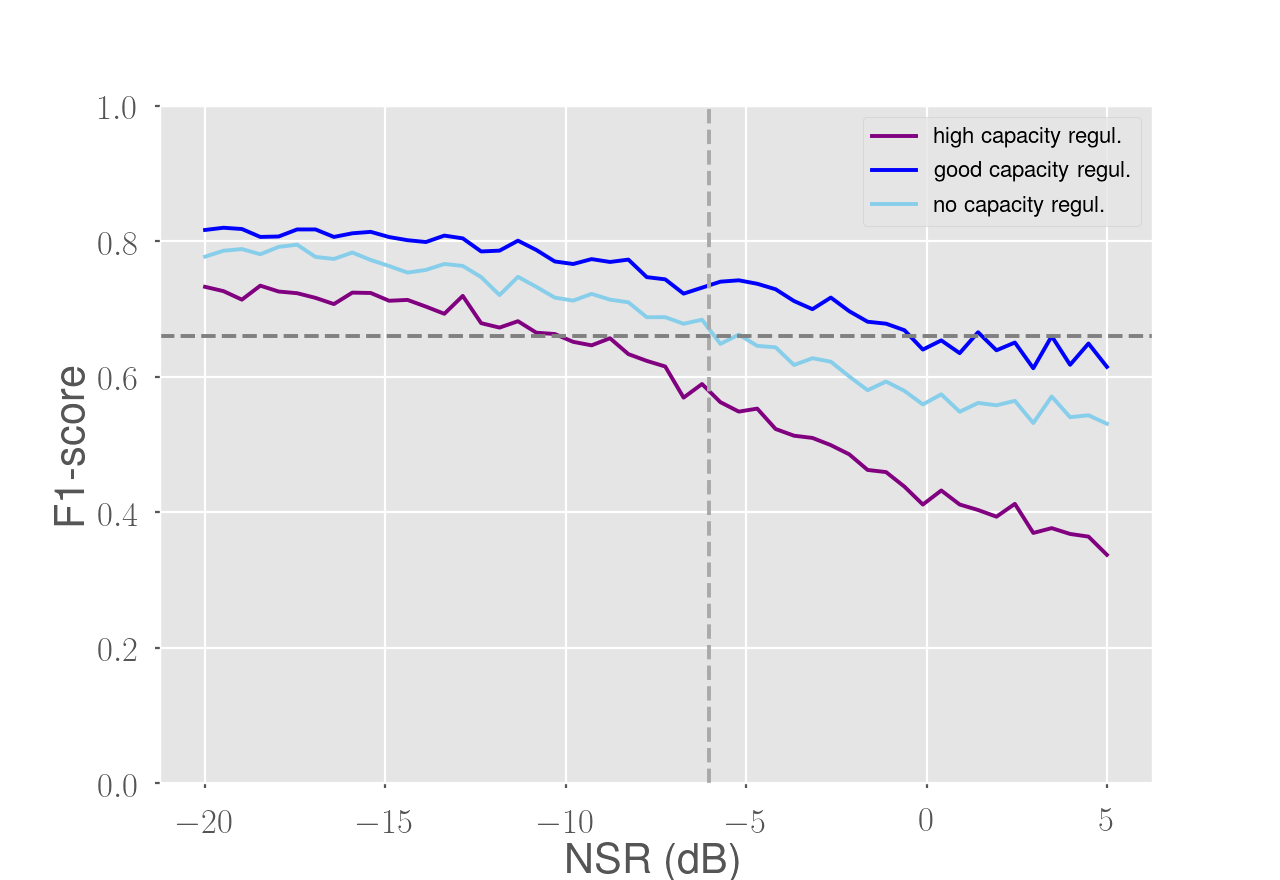
\includegraphics[scale=0.2]{figs/capacity-ip-noisy}
    \onslide<3>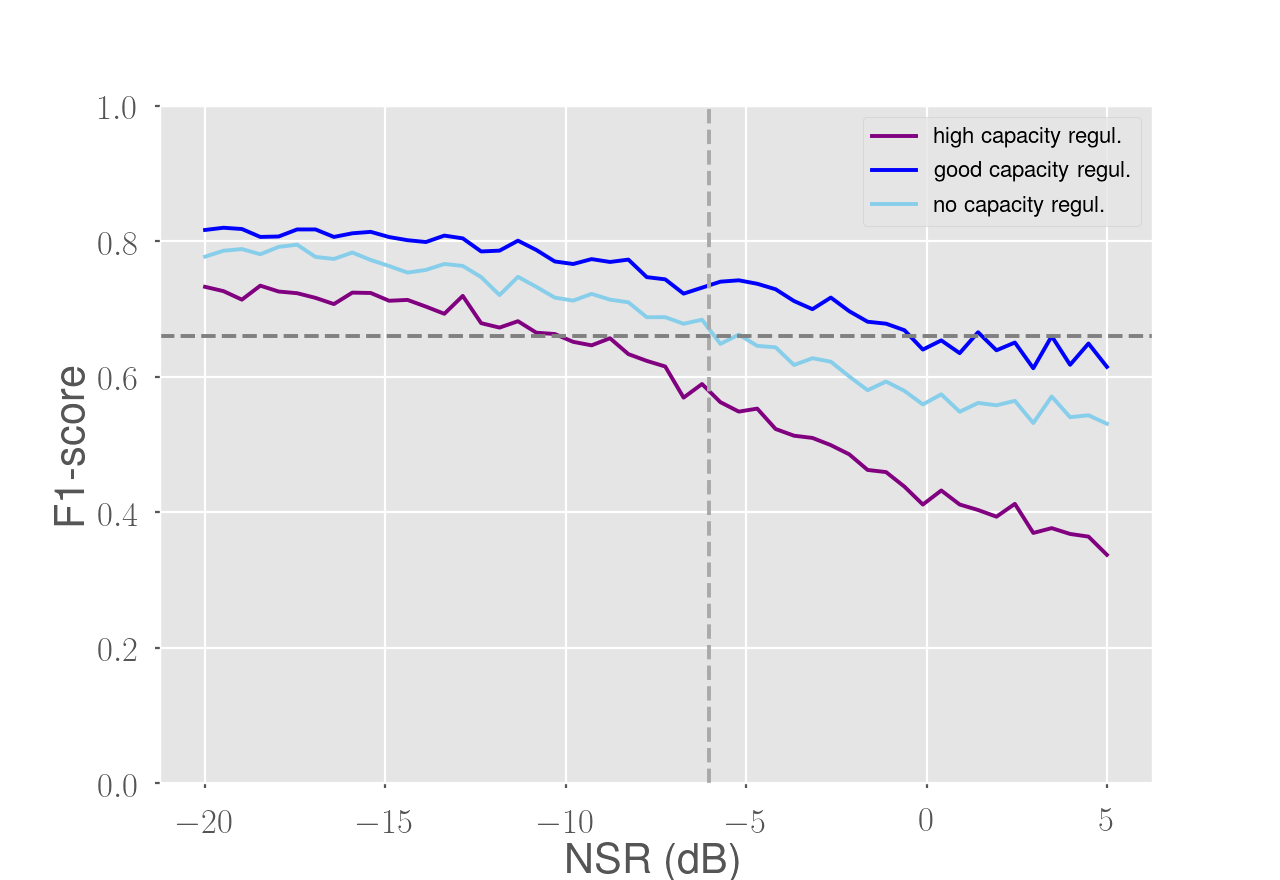
\includegraphics[scale=0.2]{figs/capacity-ip-noisy}
\end{overprint}
\caption{F1-score, noisy IP-mode}
\end{figure}
\columnbreak
\begin{figure}
\centering
\begin{overprint}
    \onslide<1>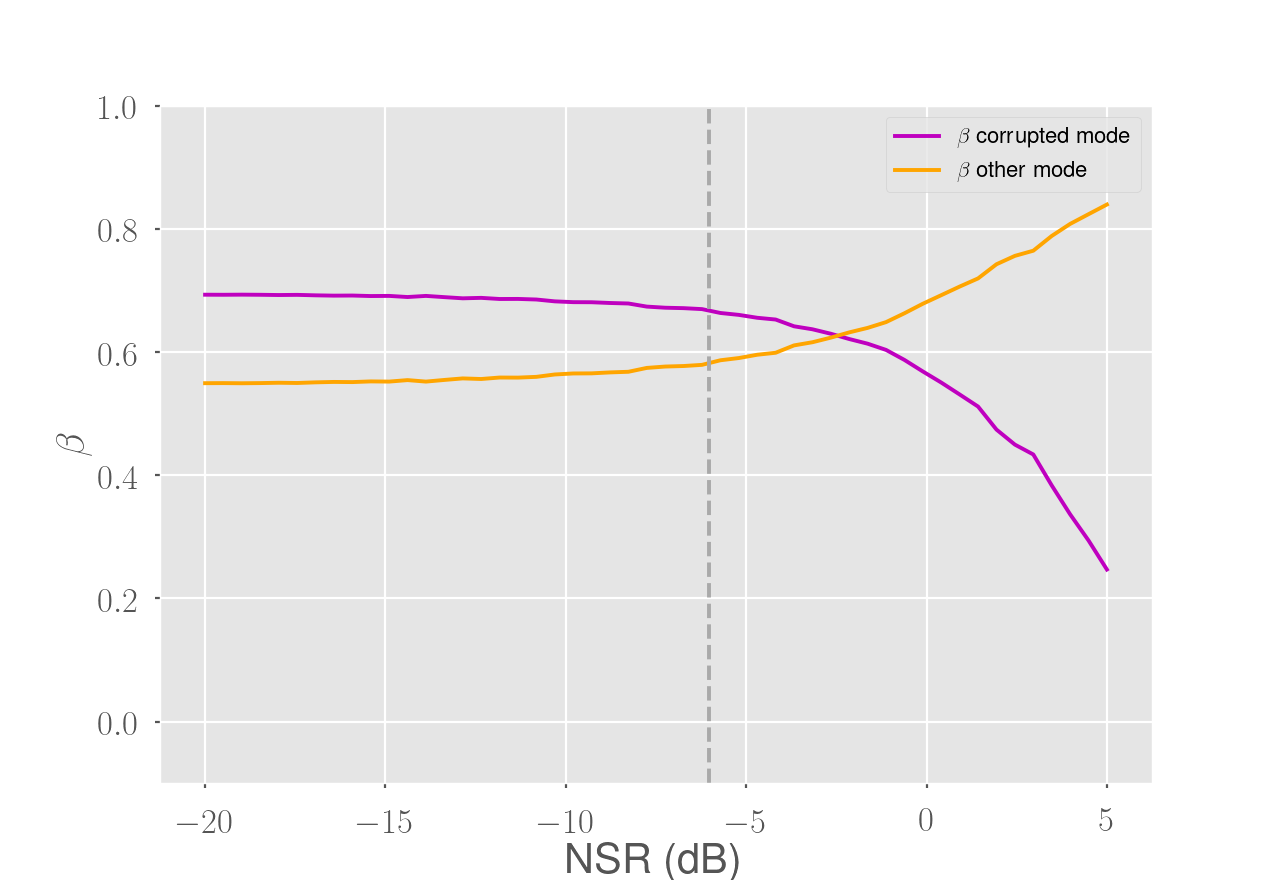
\includegraphics[scale=0.2]{figs/no-capacity-ip-noisy-beta}
    \onslide<2>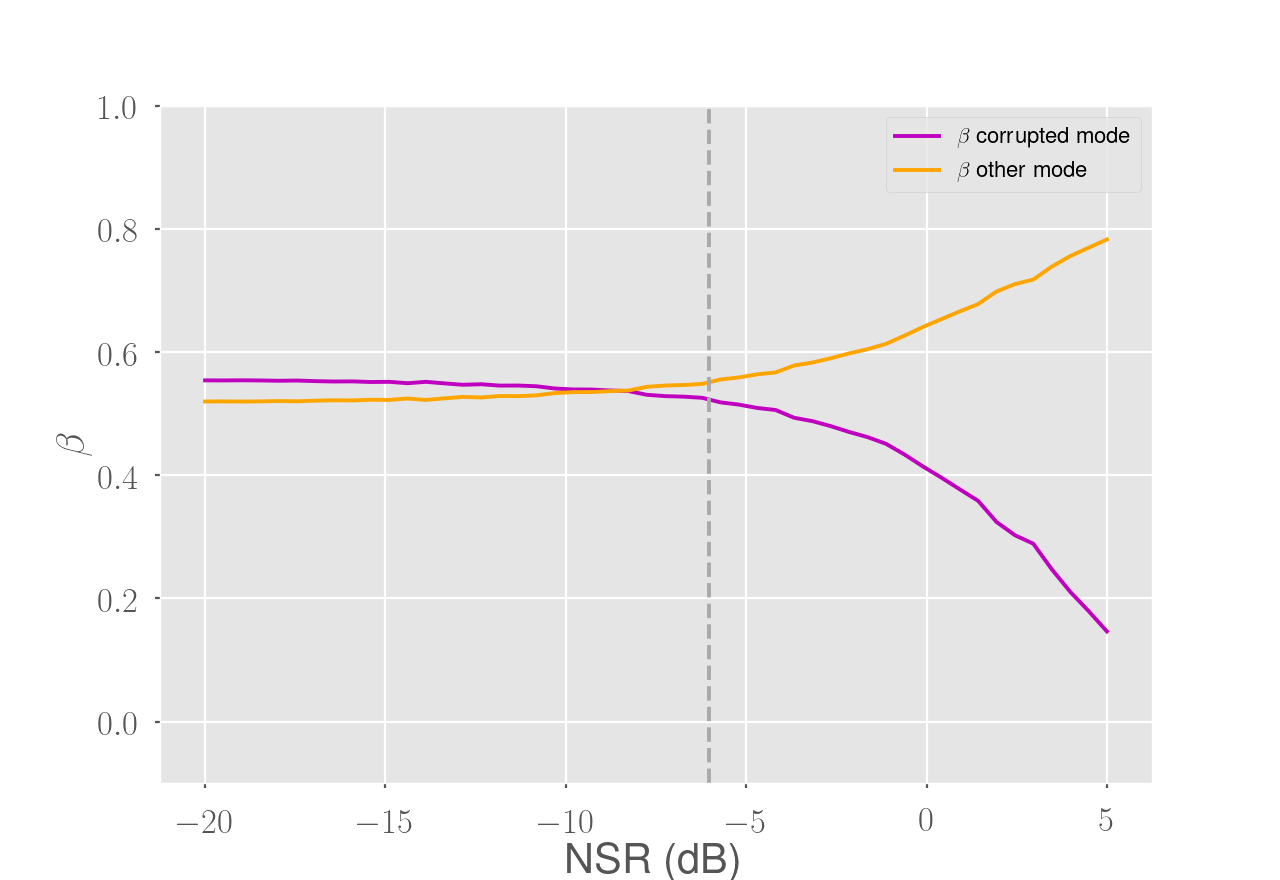
\includegraphics[scale=0.2]{figs/normal-ip-noisy-beta}
    \onslide<3>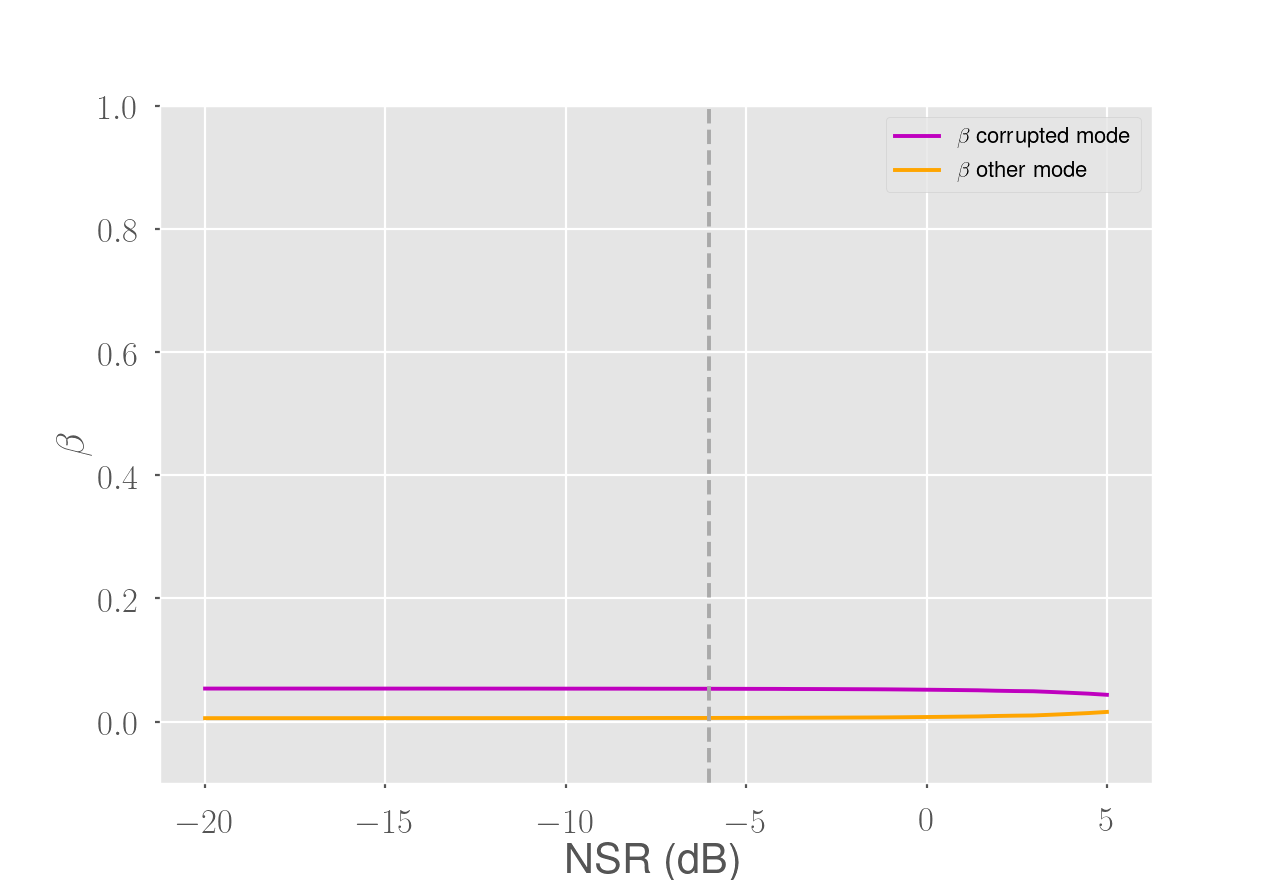
\includegraphics[scale=0.2]{figs/high-capacity-ip-noisy-beta}
\end{overprint}
\onslide<1>\caption{No capacity regularization}
\onslide<2>\vspace*{-0.9cm}\caption{Good capacity regularization}
\onslide<3>\vspace*{-0.9cm}\caption{High capacity regularization}
\end{figure}
\end{multicols}
\end{frame}


%------------------------------------------------
\begin{frame}
\frametitle{Summary}
\begin{itemize}
\item \textbf{Problem?} Failing mode(s) $\Rightarrow$ bad predictions.\vspace*{0.25cm}
\item \textbf{Hypothesis?} Some redundancy of information between the modes.\vspace*{0.25cm}
\item \textbf{Solution?} Attention module \& regularizers.\vspace*{0.25cm}
\end{itemize}
\end{frame}


\appendix
\AtBeginSection[]{
  \begin{frame}
  \vfill
  \centering
  \begin{beamercolorbox}[sep=8pt,center,shadow=true,rounded=true]{title}
    \usebeamerfont{title}\insertsectionhead\par%
  \end{beamercolorbox}
  \vfill
  \end{frame}
}
\section{Backup slides}

%------------------------------------------------
\begin{frame}
\frametitle{Influence of energy regularizer}
\begin{multicols}{2}
\begin{figure}
\centering
\begin{overprint}
    \onslide<1>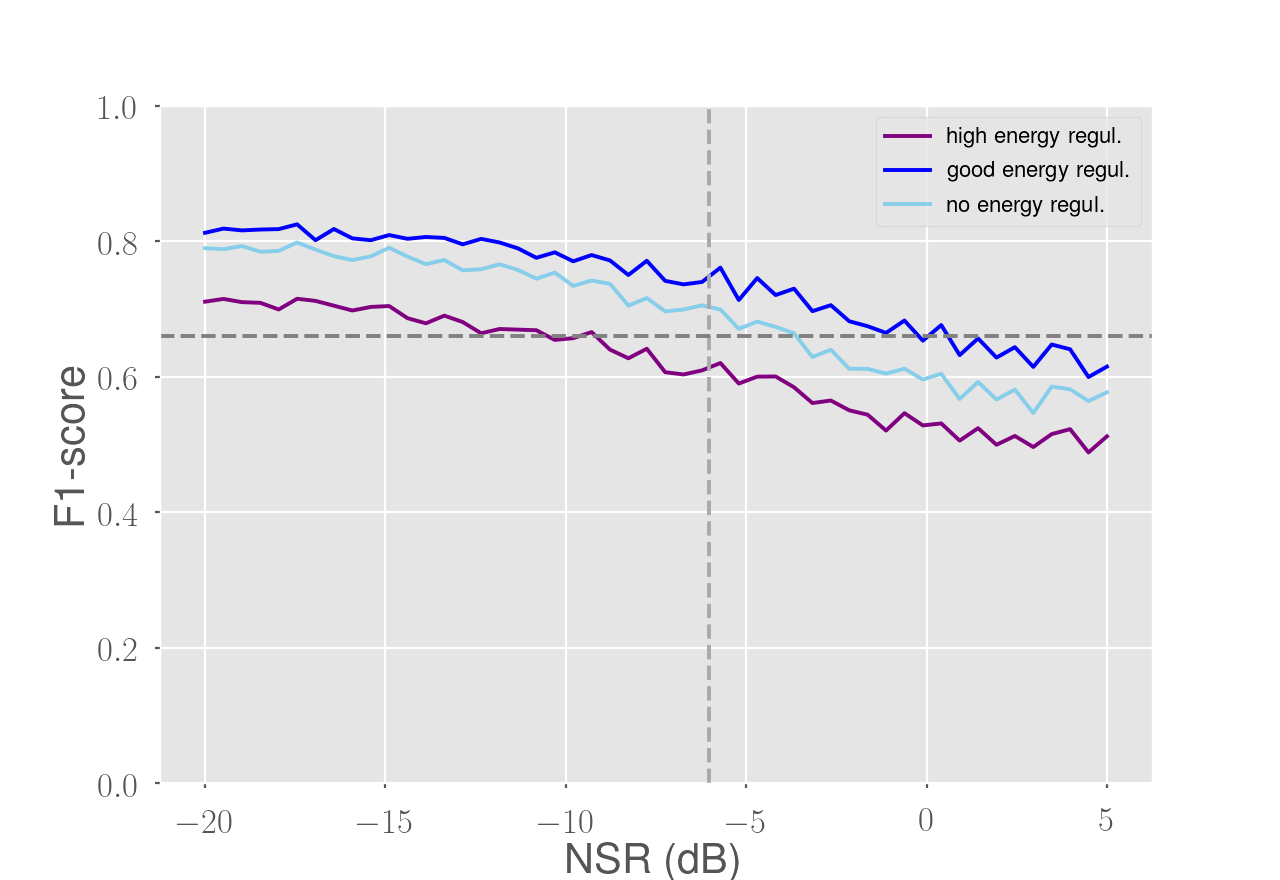
\includegraphics[scale=0.2]{figs/energy-ip-noisy}
    \onslide<2>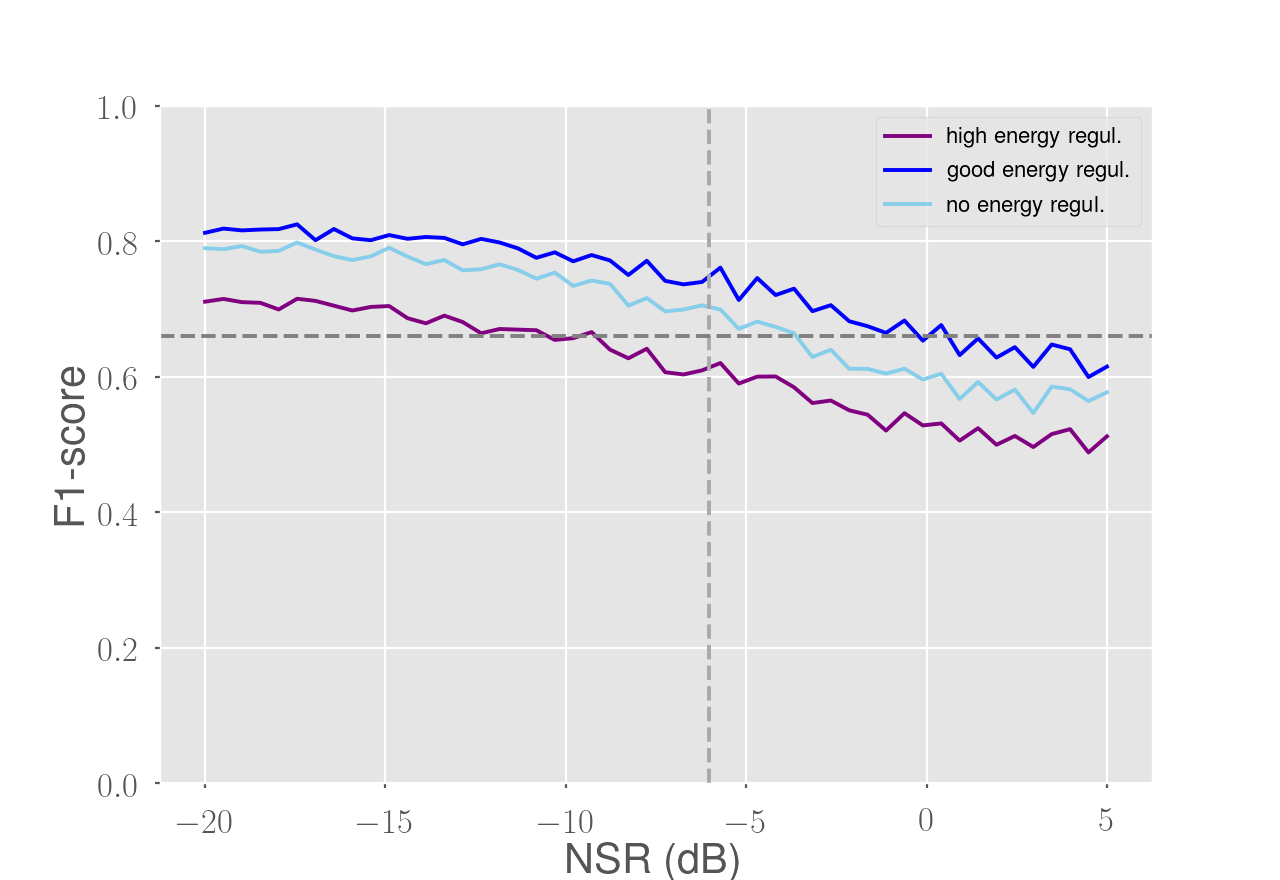
\includegraphics[scale=0.2]{figs/energy-ip-noisy}
    \onslide<3>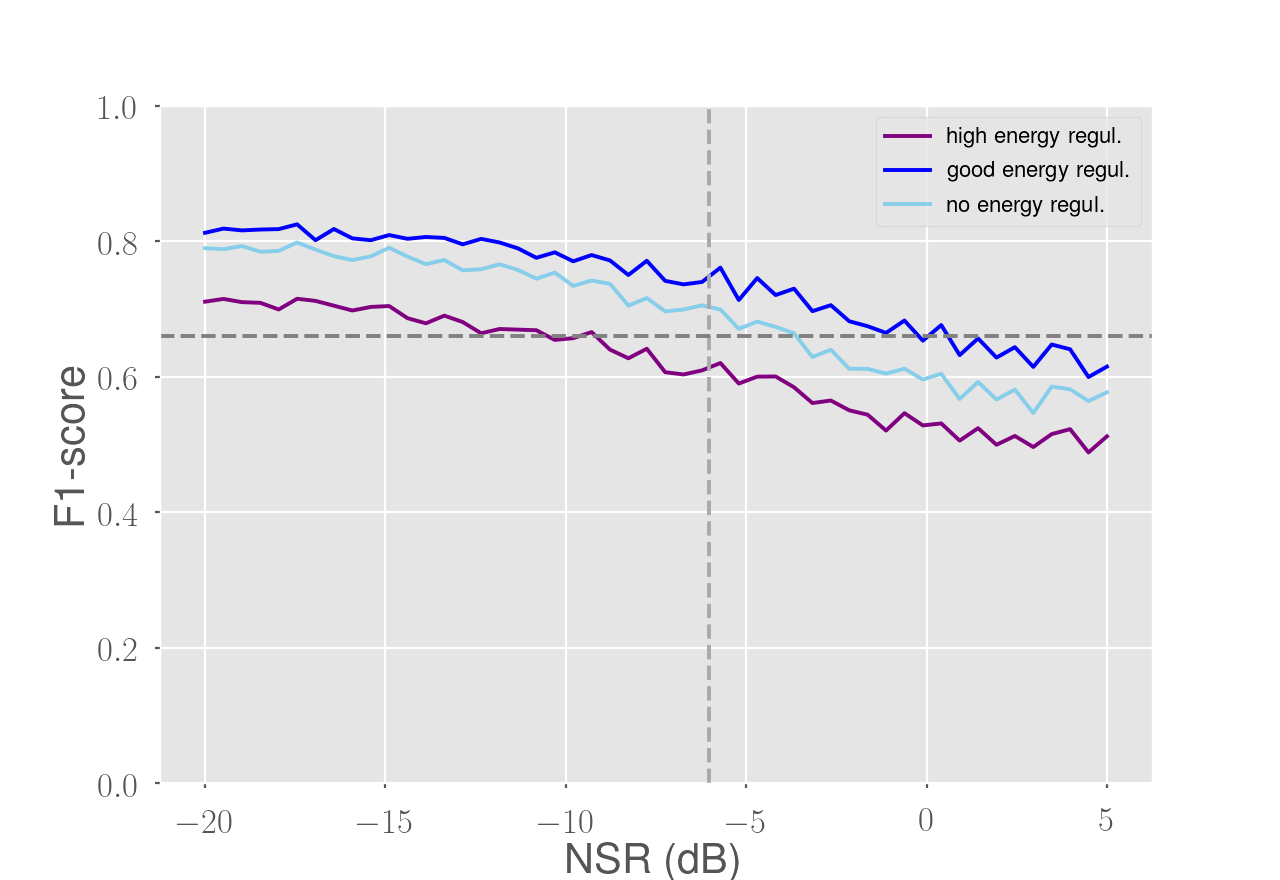
\includegraphics[scale=0.2]{figs/energy-ip-noisy}
\end{overprint}
\caption{F1-score, noisy IP-mode}
\end{figure}
\columnbreak
\begin{figure}
\centering
\begin{overprint}
    \onslide<1>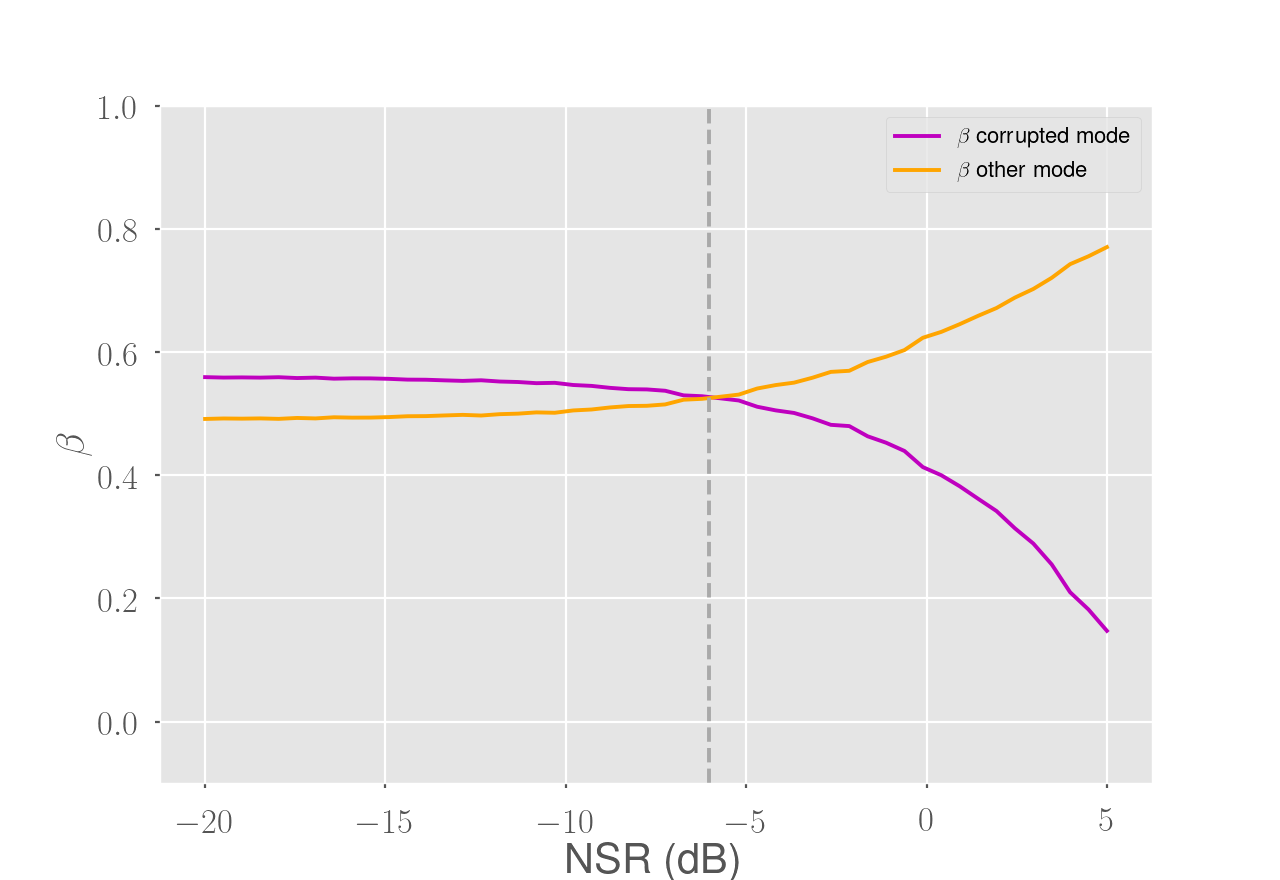
\includegraphics[scale=0.2]{figs/no-energy-ip-noisy-beta}
    \onslide<2>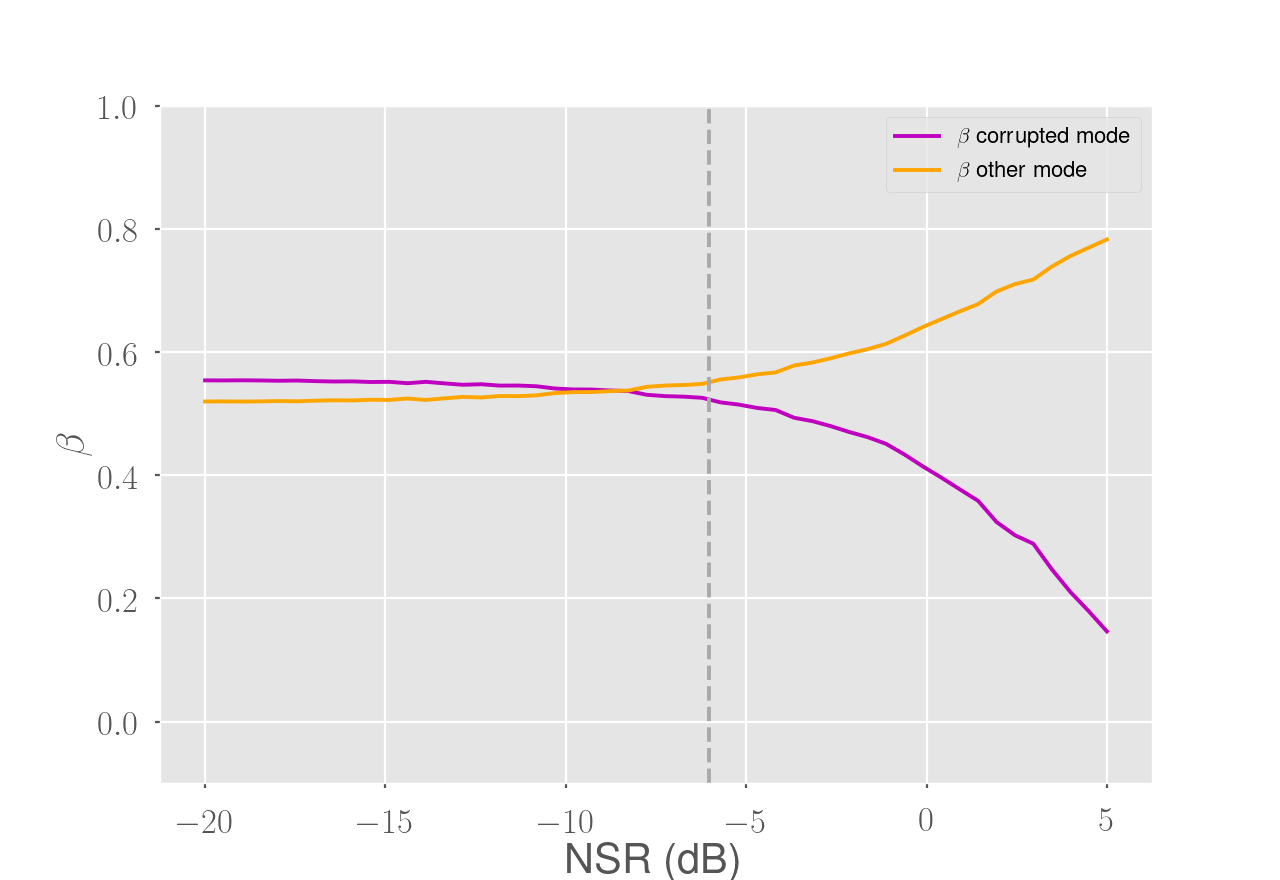
\includegraphics[scale=0.2]{figs/normal-ip-noisy-beta}
    \onslide<3>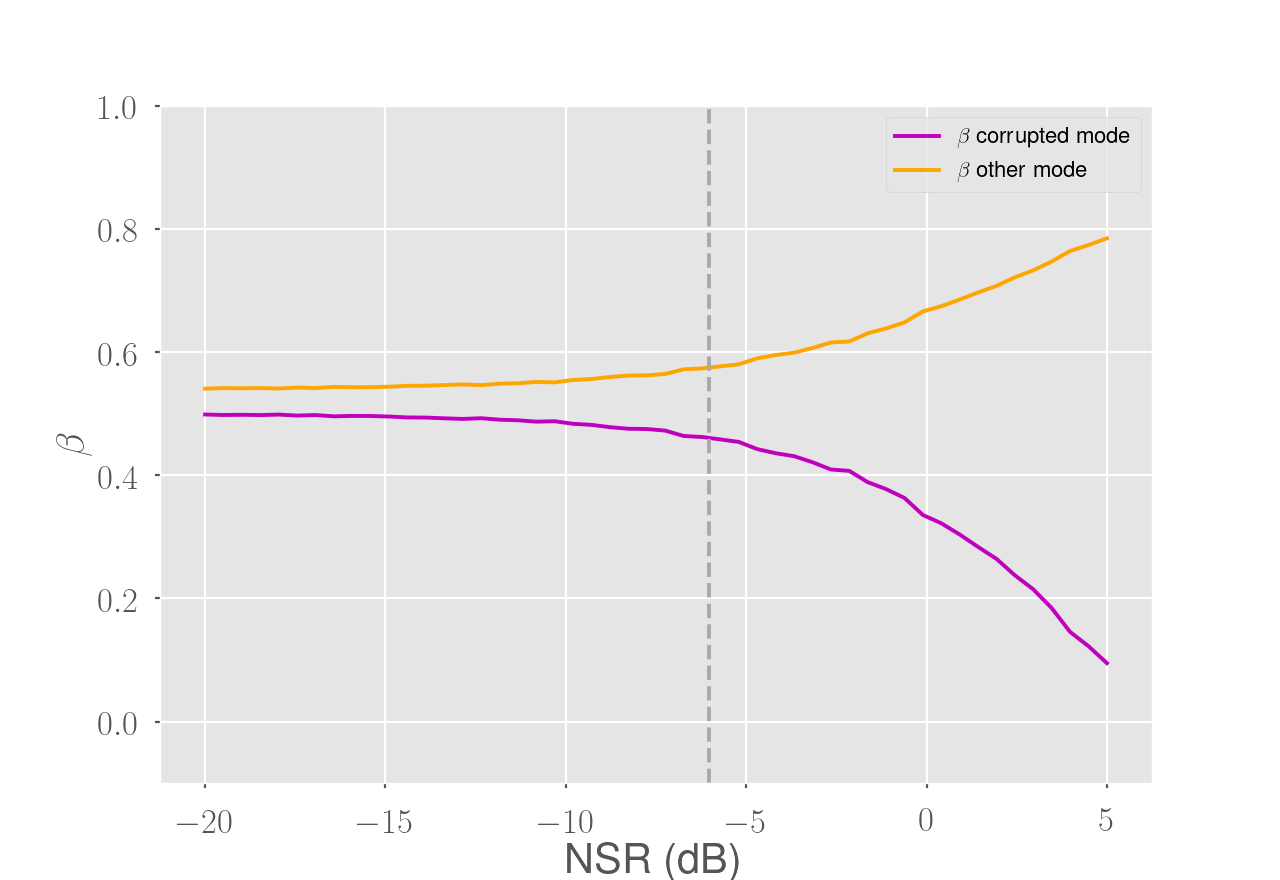
\includegraphics[scale=0.2]{figs/high-energy-ip-noisy-beta}
\end{overprint}
\onslide<1>\caption{No energy regularization}
\onslide<2>\vspace*{-0.9cm}\caption{Good energy regularization}
\onslide<3>\vspace*{-0.9cm}\caption{High energy regularization}
\end{figure}
\end{multicols}
\end{frame}

%------------------------------------------------
\begin{frame}
\frametitle{Influence of energy regularizer for DM mode}
\begin{multicols}{2}
\begin{figure}
\centering
\begin{overprint}
    \onslide<1>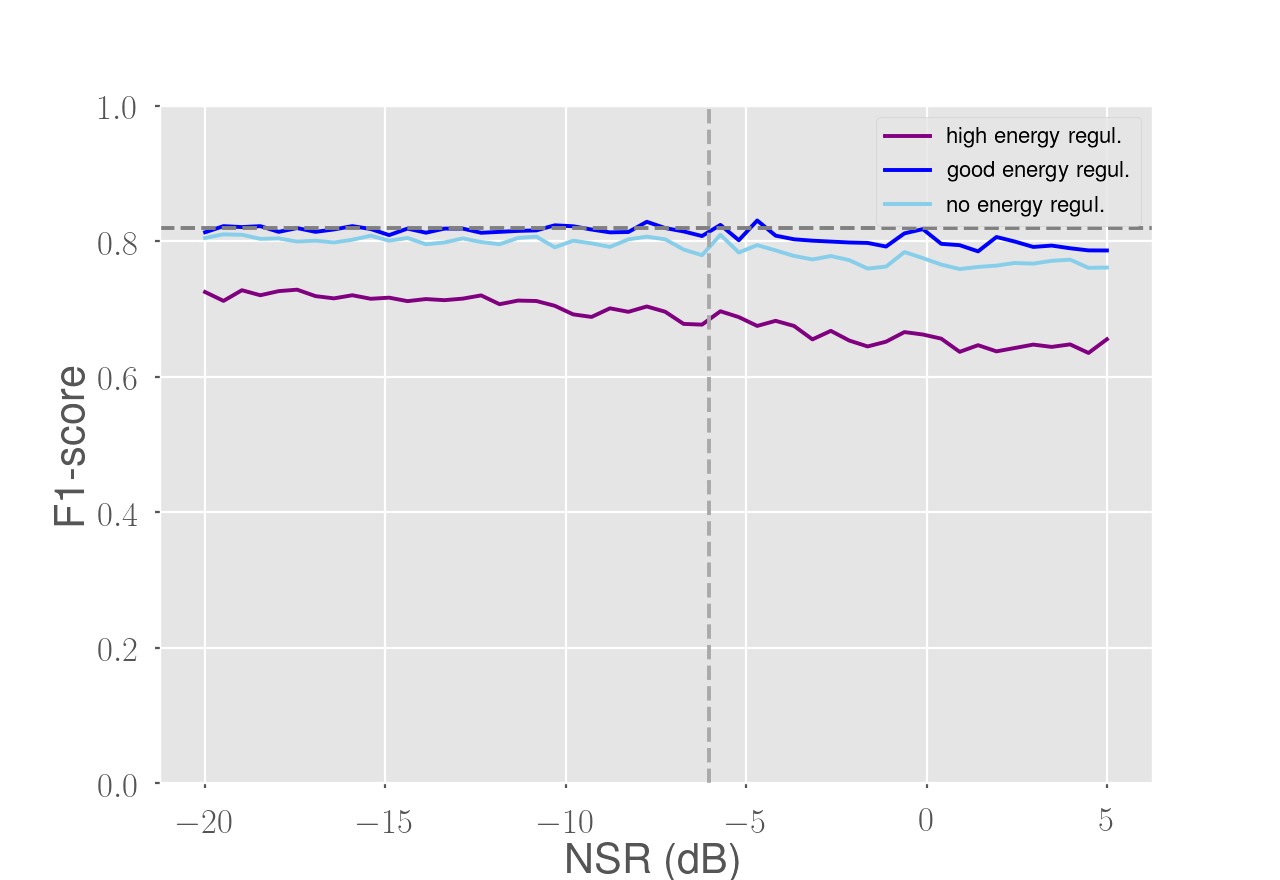
\includegraphics[scale=0.2]{figs/energy-dm-noisy}
    \onslide<2>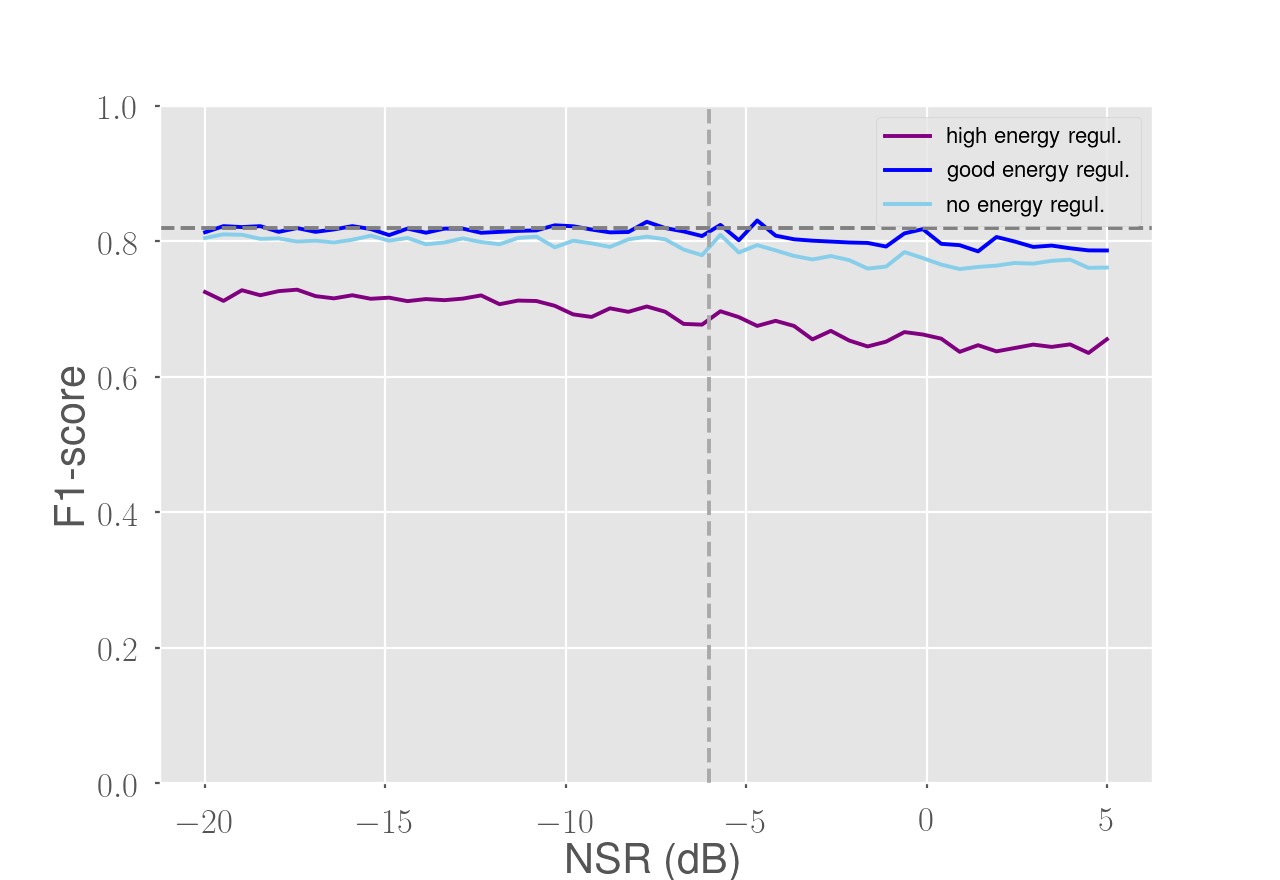
\includegraphics[scale=0.2]{figs/energy-dm-noisy}
    \onslide<3>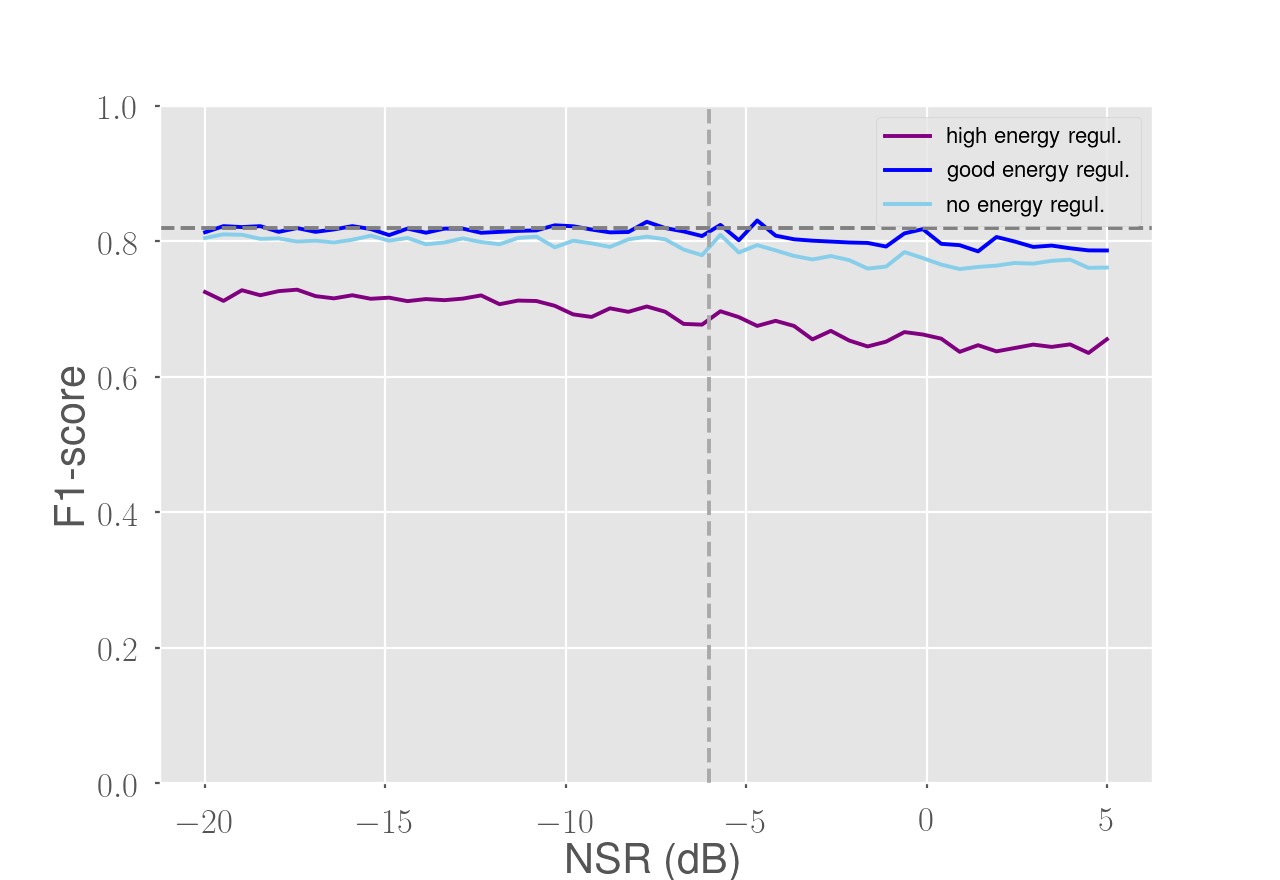
\includegraphics[scale=0.2]{figs/energy-dm-noisy}
\end{overprint}
\caption{F1-score, noisy IP-mode}
\end{figure}
\columnbreak
\begin{figure}
\centering
\begin{overprint}
    \onslide<1>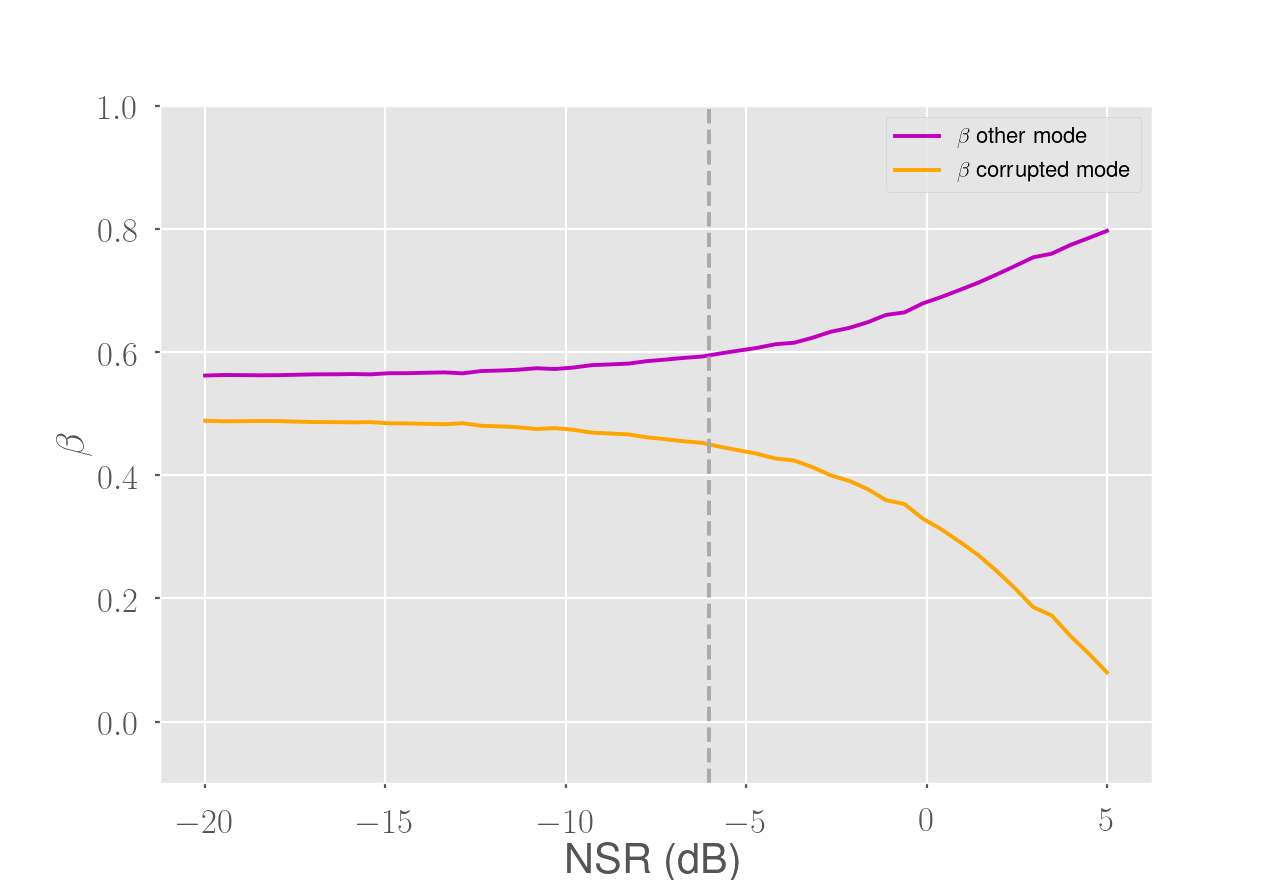
\includegraphics[scale=0.2]{figs/no-energy-dm-noisy-beta}
    \onslide<2>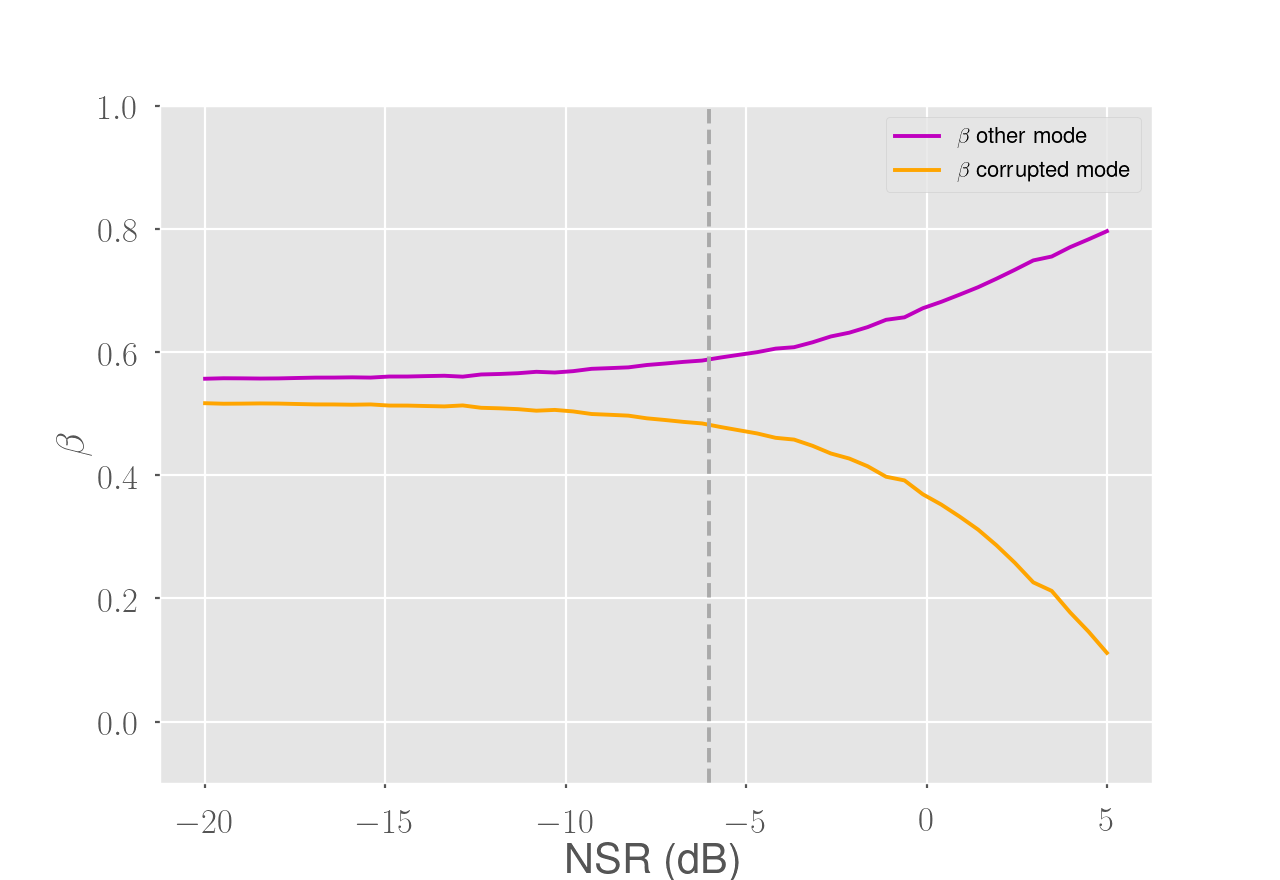
\includegraphics[scale=0.2]{figs/normal-dm-noisy-beta}
    \onslide<3>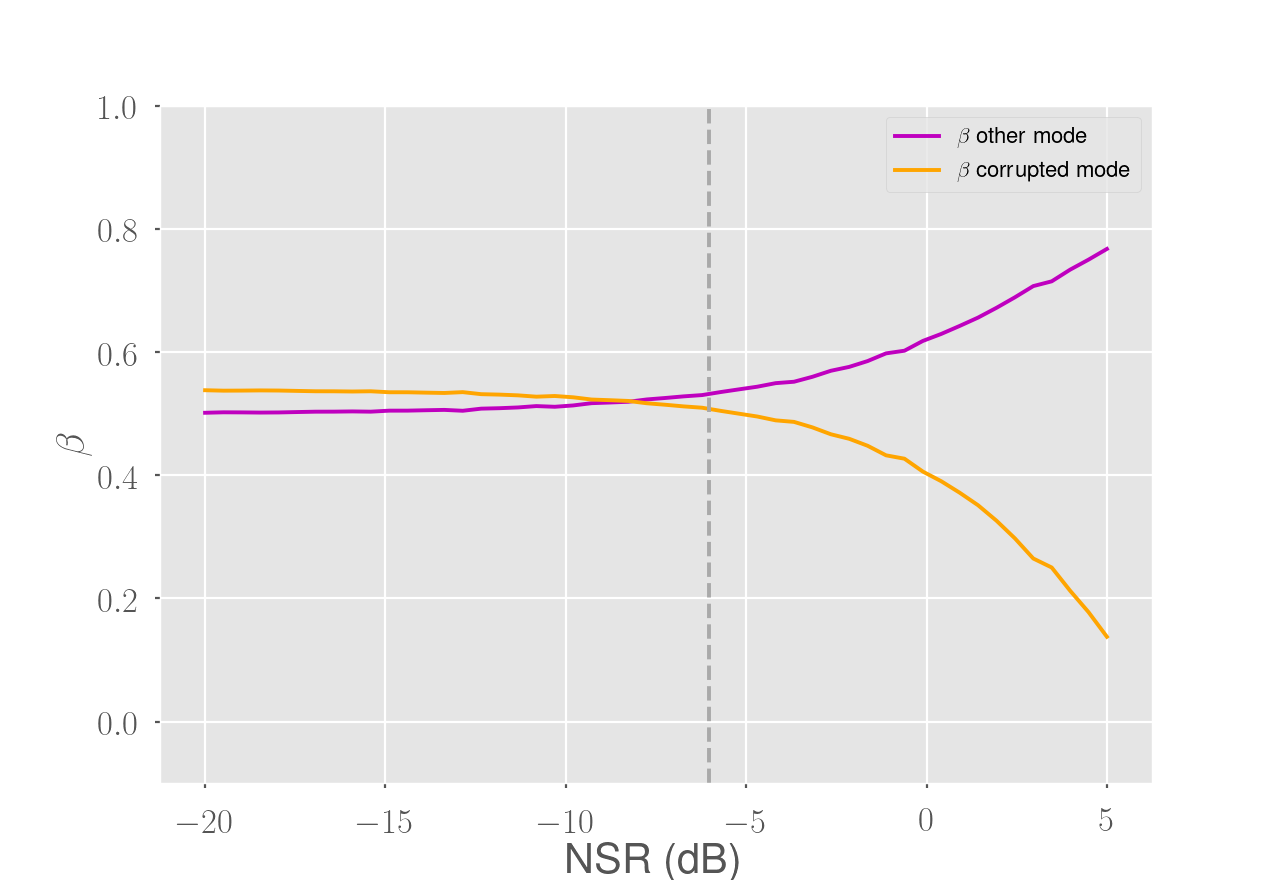
\includegraphics[scale=0.2]{figs/high-energy-dm-noisy-beta}
\end{overprint}
\onslide<1>\caption{No energy regularization}
\onslide<2>\vspace*{-0.9cm}\caption{Good energy regularization}
\onslide<3>\vspace*{-0.9cm}\caption{High energy regularization}
\end{figure}
\end{multicols}
\end{frame}

%------------------------------------------------
\begin{frame}
\frametitle{Influence of capacity minimization for DM mode}
\begin{multicols}{2}
\begin{figure}
\centering
\begin{overprint}
    \onslide<1>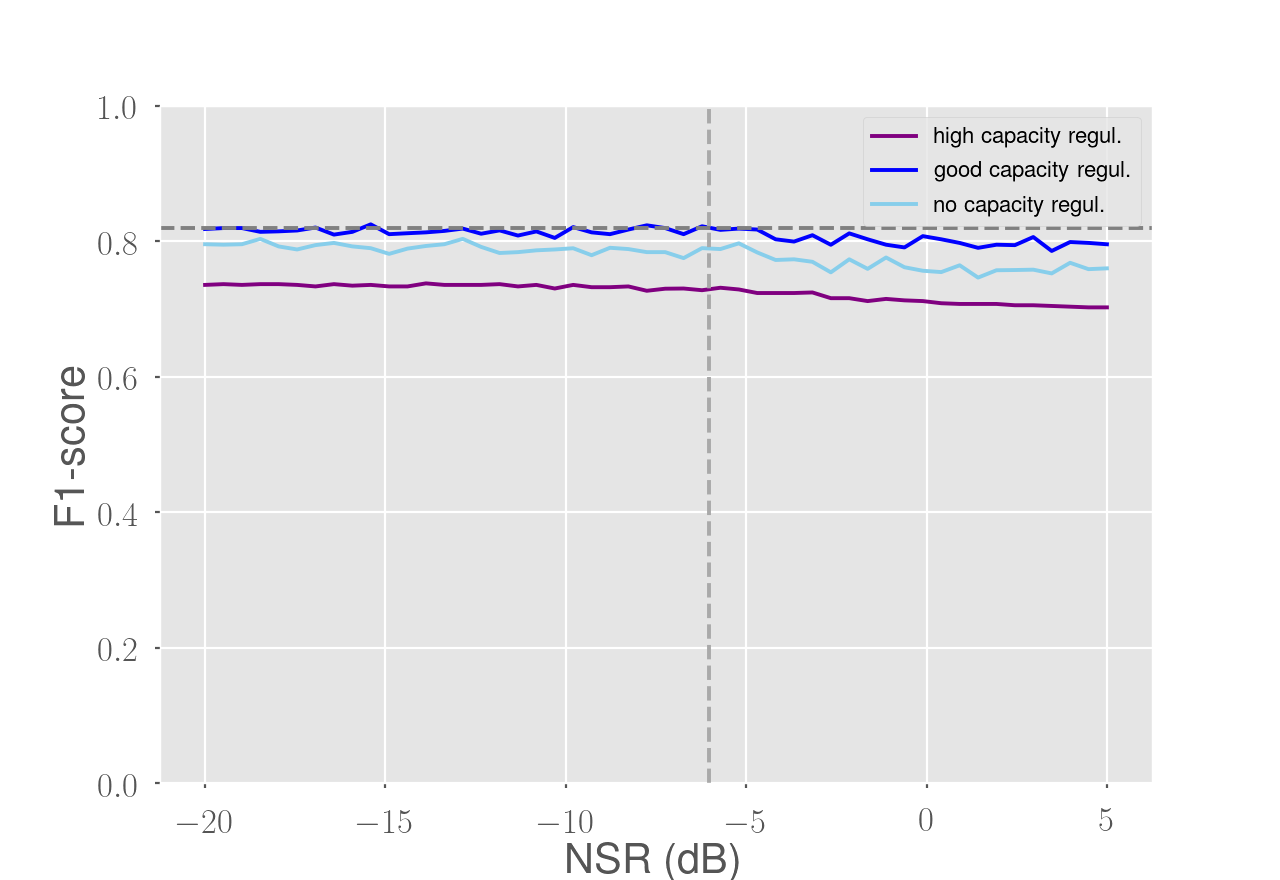
\includegraphics[scale=0.2]{figs/capacity-dm-noisy}
    \onslide<2>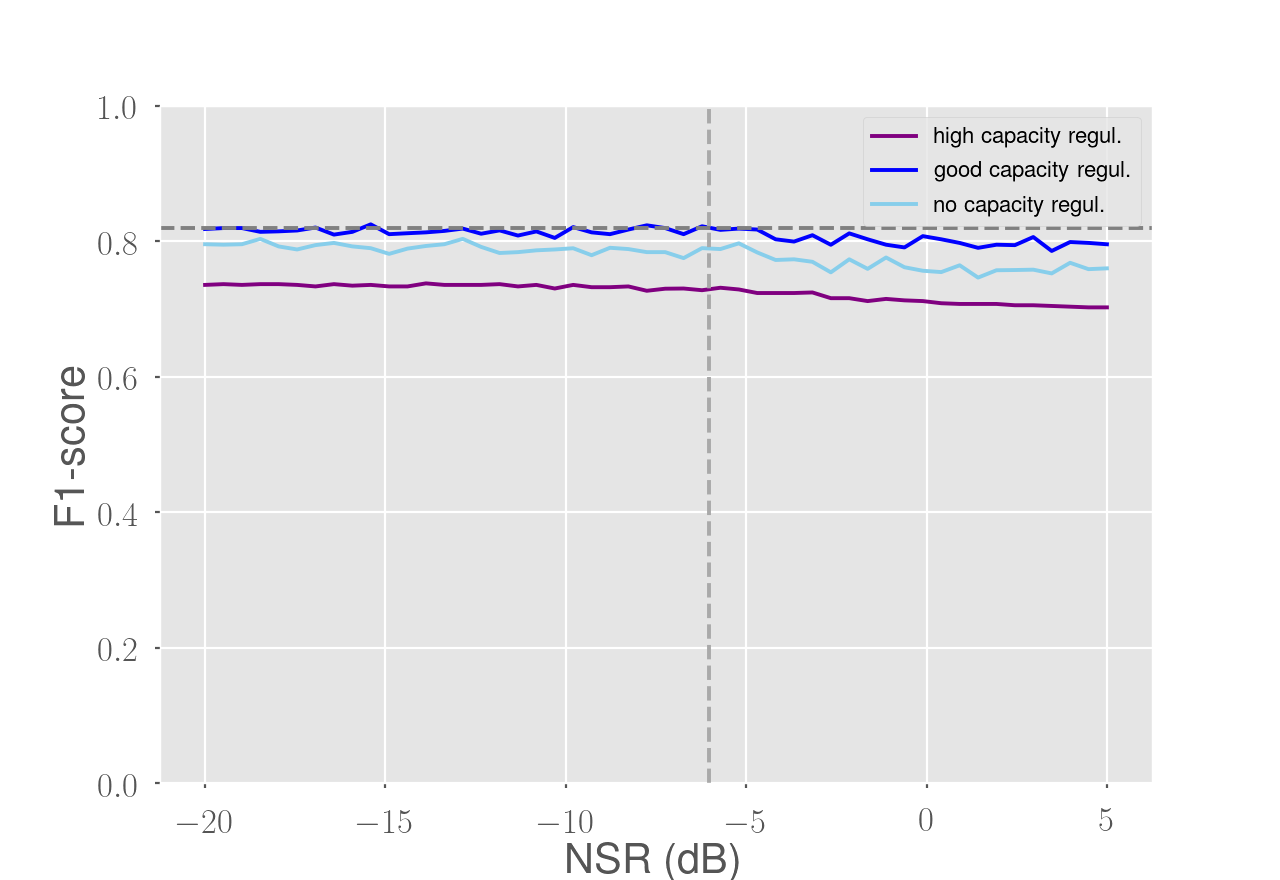
\includegraphics[scale=0.2]{figs/capacity-dm-noisy}
    \onslide<3>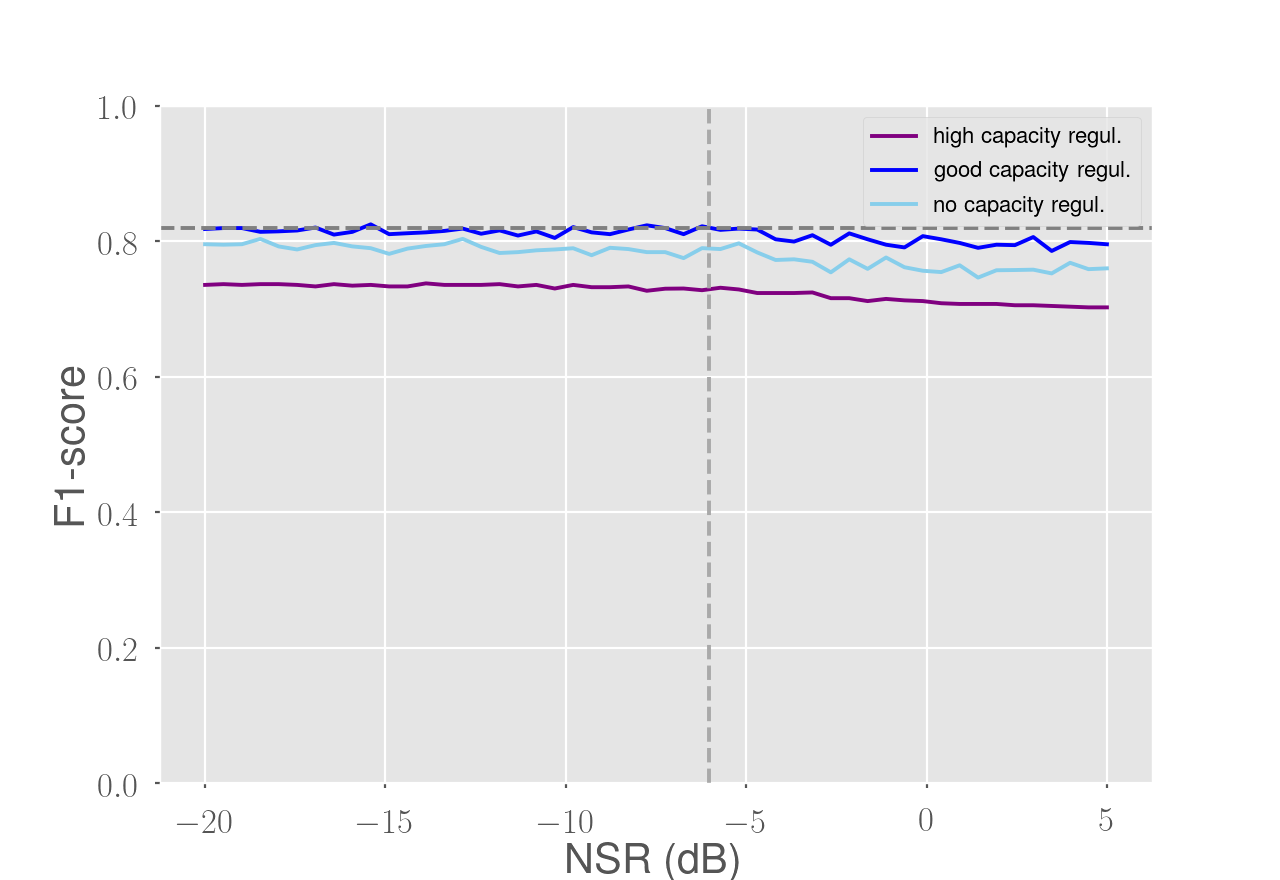
\includegraphics[scale=0.2]{figs/capacity-dm-noisy}
\end{overprint}
\caption{F1-score, noisy IP-mode}
\end{figure}
\columnbreak
\begin{figure}
\centering
\begin{overprint}
    \onslide<1>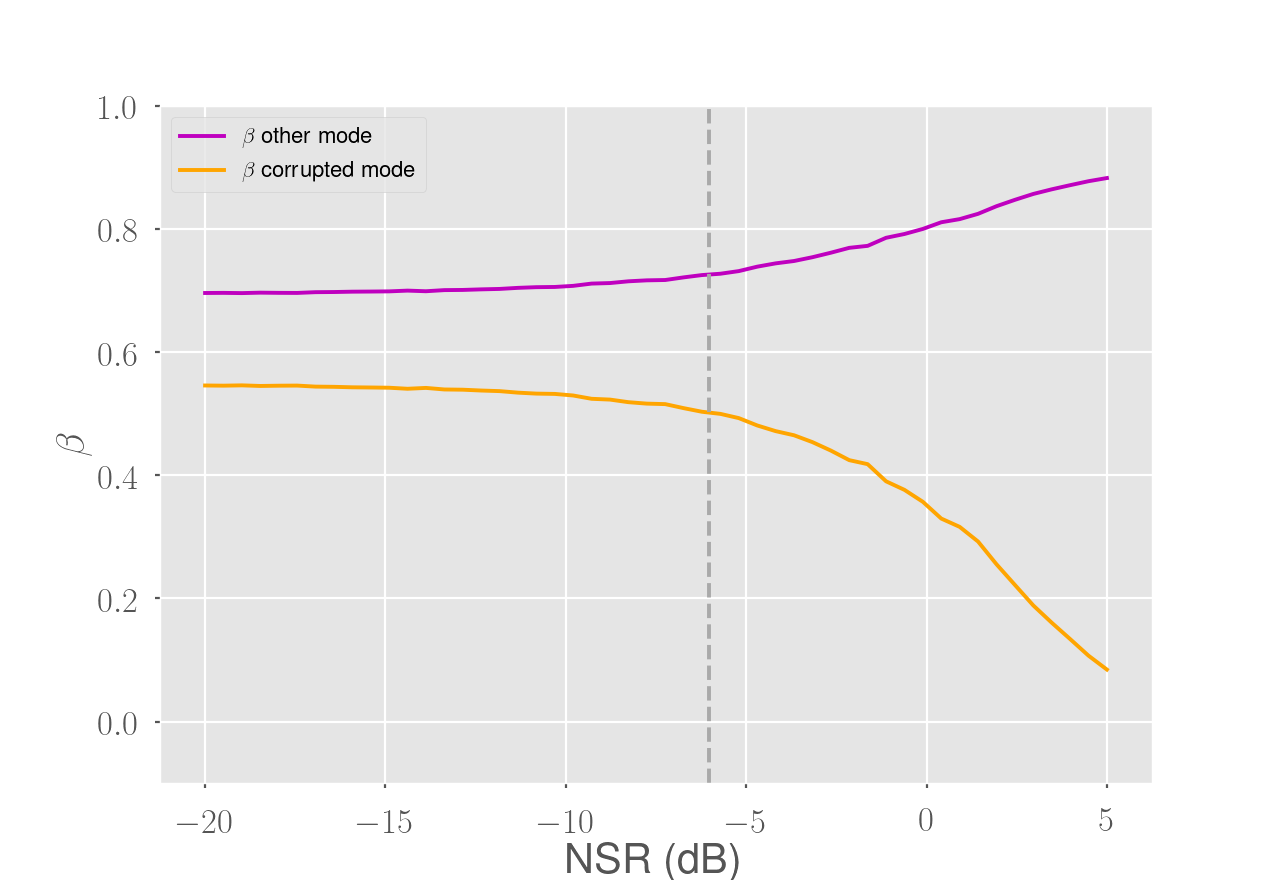
\includegraphics[scale=0.2]{figs/no-capacity-dm-noisy-beta}
    \onslide<2>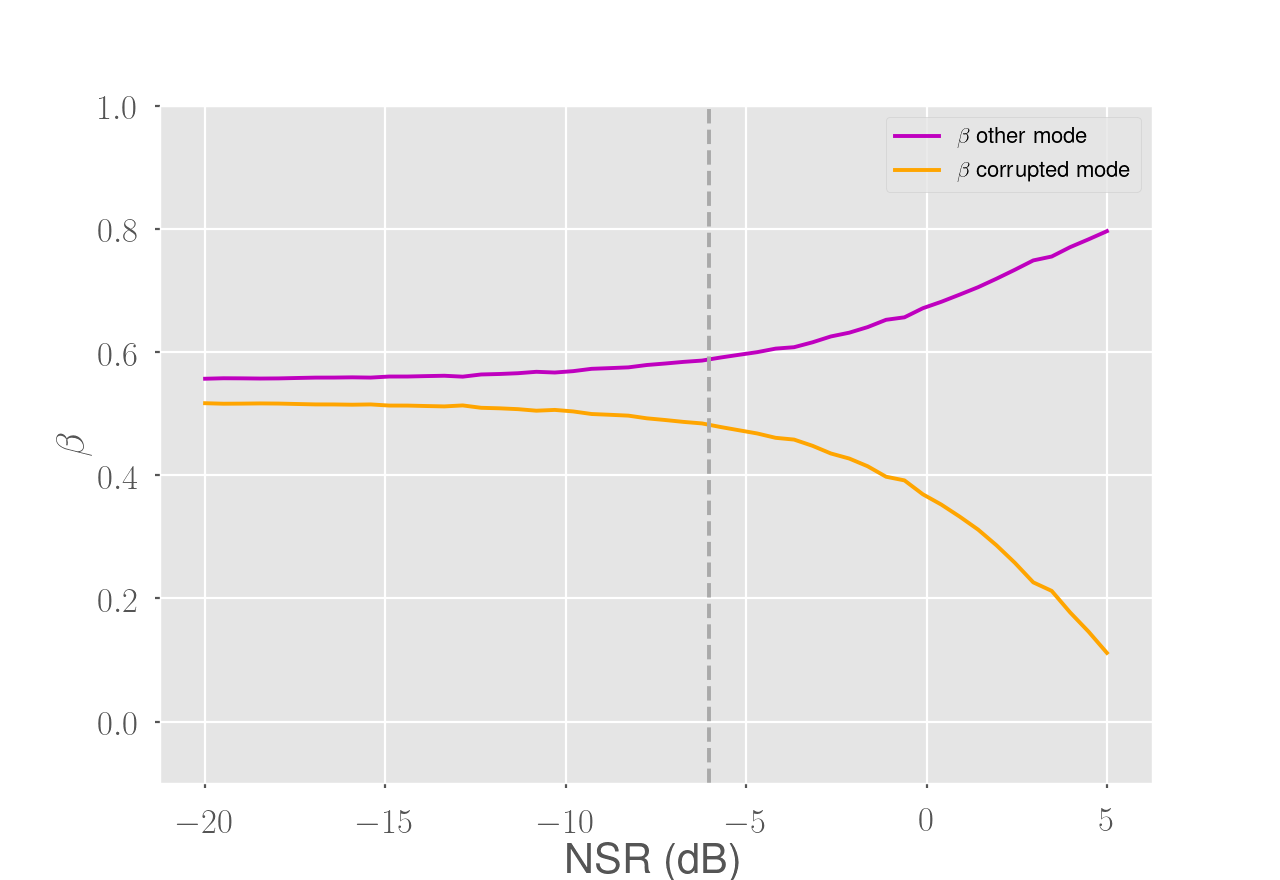
\includegraphics[scale=0.2]{figs/normal-dm-noisy-beta}
    \onslide<3>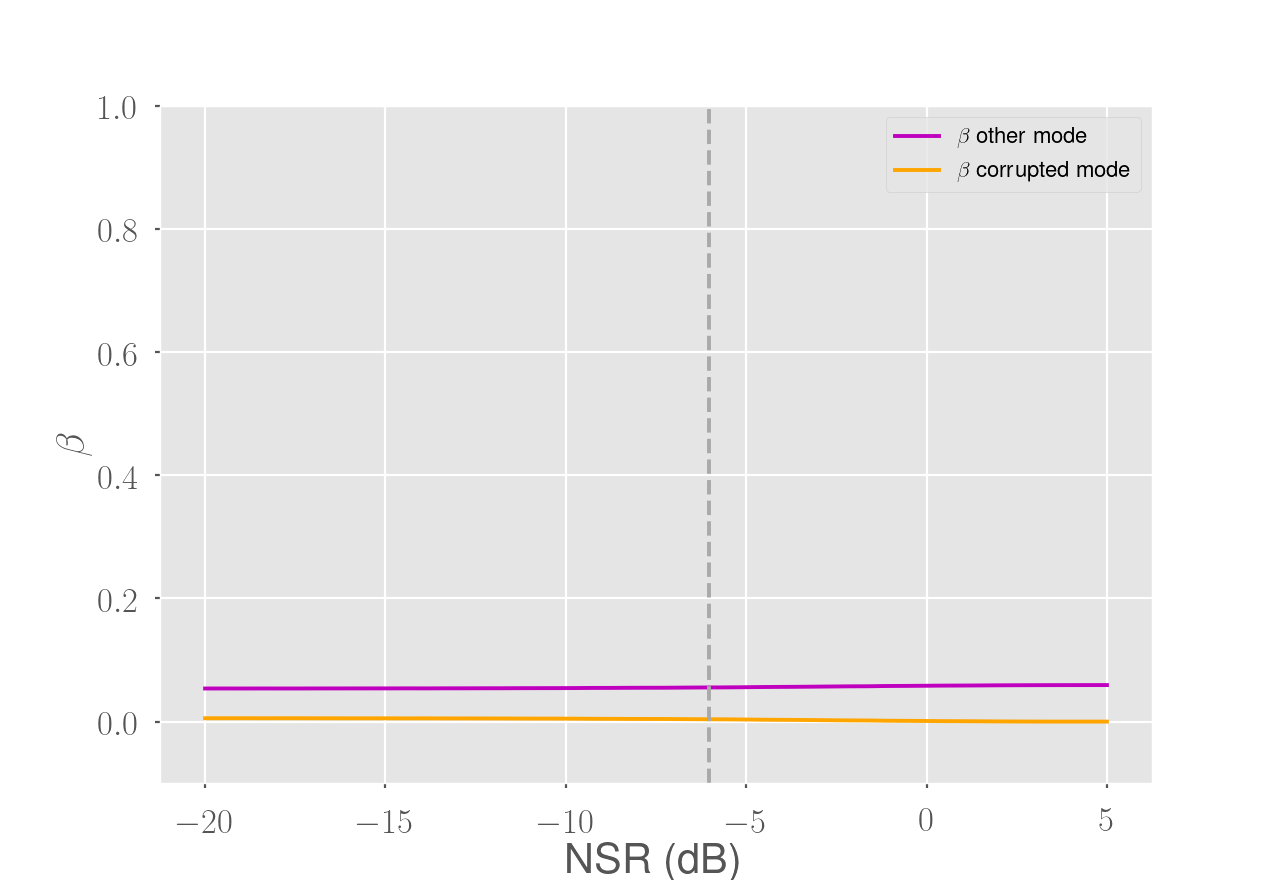
\includegraphics[scale=0.2]{figs/high-capacity-dm-noisy-beta}
\end{overprint}
\onslide<1>\caption{No capacity regularization}
\onslide<2>\vspace*{-0.9cm}\caption{Good capacity regularization}
\onslide<3>\vspace*{-0.9cm}\caption{High capacity regularization}
\end{figure}
\end{multicols}
\end{frame}

%------------------------------------------------
\begin{frame}
\frametitle{General framework}
\begin{enumerate}
\item Failure intensity, $\Psi_i$ \vspace*{0.35cm}
\item Self-energy, $e_i = w_i\Psi_i + b_i$ \vspace*{0.35cm}
\item Shared energies, $e_{ij} = w_{ij}e_i^{\gamma_{ij}}e_j^{1-\gamma_{ij}}$ \vspace*{0.35cm}
\item Modal energy, $E_i = e_i + \sum_{j\neq i} e_{ij}$ \vspace*{0.35cm}
\item Importance score, $\alpha_i = \frac{1}{Z}e^{-\rho E_i}$ \vspace*{0.35cm}
\item Attention score, $\beta_i = \max[0, \tanh(g_a\alpha_i - b_a)]$ \vspace*{0.35cm}
\end{enumerate}
\end{frame}

%------------------------------------------------
\begin{frame}
\frametitle{Capacity minimization}
\begin{equation}
\tilde{\mathcal{L}} = \mathcal{L}(y,\hat{y}) + \lambda_c(g_a-b_a)
\end{equation}
\begin{figure}
\centering
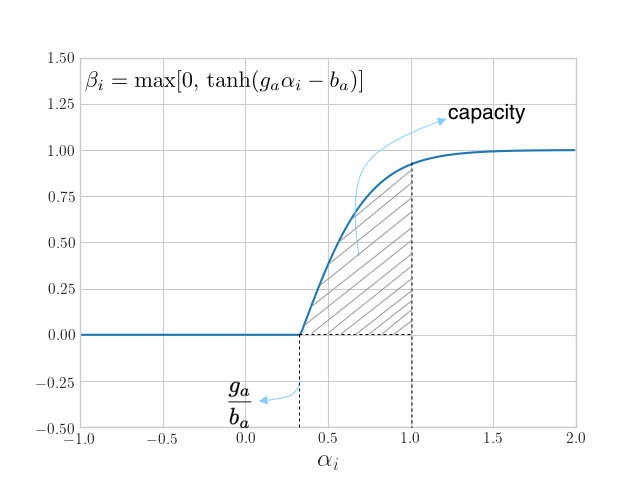
\includegraphics[scale=0.3]{figs/tanh-annotated}
\caption{Attention function}
\label{fig:attention-function}
\end{figure}
\end{frame}

%------------------------------------------------
\begin{frame}
\frametitle{Discrepancy minimization (Definition)}
\begin{equation}
\tilde{\mathcal{L}} = \mathcal{L}(y,\hat{y}) - \lambda_e \Omega
\end{equation}
\begin{center}
with\end{center}
 \begin{equation}
 \Omega = \sum_{k=1}^M \xi_k \log(\alpha_k) \quad \text{and} \quad \xi_k = \begin{cases}
      \xi_- = -1 & \text{if}\ \mathbf{x}_k\, \text{is corrupted} \\
      \xi_+ = +1 & \text{otherwise}
    \end{cases}
\end{equation}
\end{frame}


%------------------------------------------------
\begin{frame}
\frametitle{Discrepancy minimization (Result)}
If $M$ is even,
\begin{equation}
E_i\big(\mathbf{x}_i;\bm{\theta}_i^{(0)} - \epsilon\lambda_e\rho\xi_i\nabla_{\bm{\theta}_i}E_i\big) \approx E_i\big(\mathbf{x}_i;\bm{\theta}_i^{(0)}\big) - \epsilon\lambda_e\rho\xi_i\big(\nabla_{\bm{\theta}_i}E_i\big)^T\nabla_{\bm{\theta}_i}E_i
\end{equation}
If $M$ is uneven,
\begin{equation}
\bm{\theta}_i \leftarrow \begin{cases}
       \bm{\theta}_i - \epsilon\lambda_e\rho(1-\alpha_i)\nabla_{\bm{\theta}_i}E_i, & \text{if $i$ is uncorrupted} \\
       \bm{\theta}_i + \epsilon\lambda_e\rho(1+\alpha_i)\nabla_{\bm{\theta}_i}E_i & \text{otherwise}
    \end{cases}
\end{equation}
\end{frame}

%------------------------------------------------
\begin{frame}
\frametitle{Multiple noisy modes}
\begin{multicols}{2}
\begin{figure}
\centering
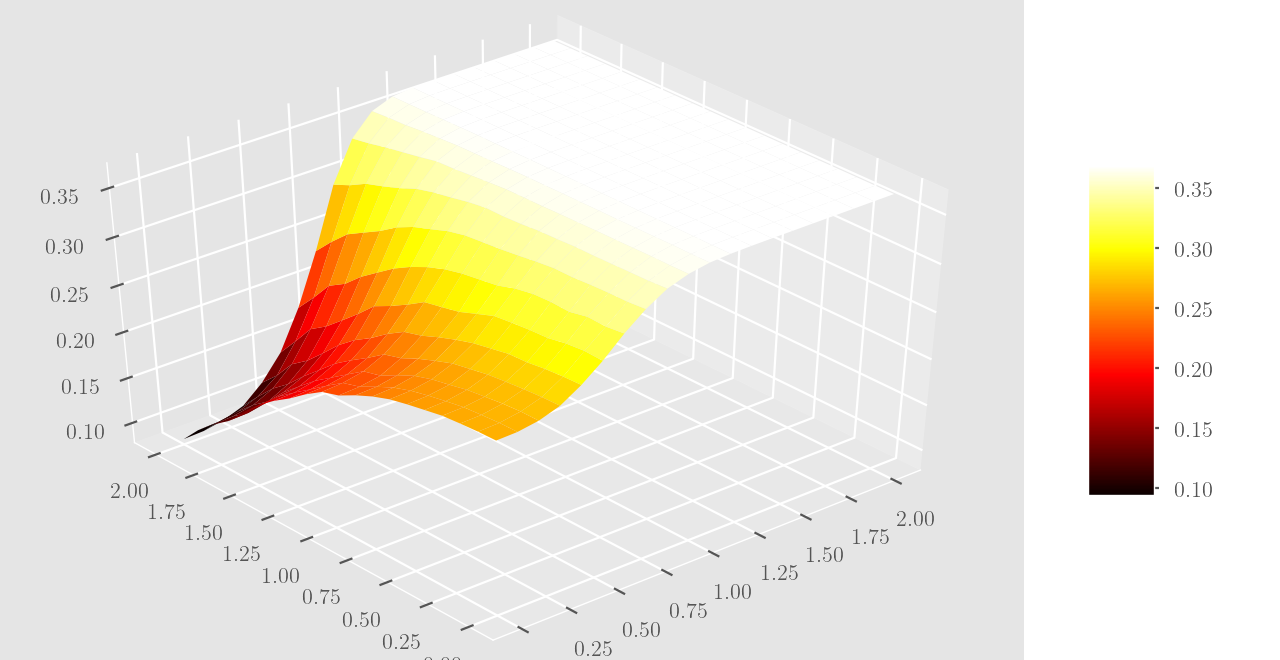
\includegraphics[scale=0.18]{figs/Figure_1} 
  \caption{$\beta$-IP}
\end{figure}
\columnbreak
\begin{figure}
\centering
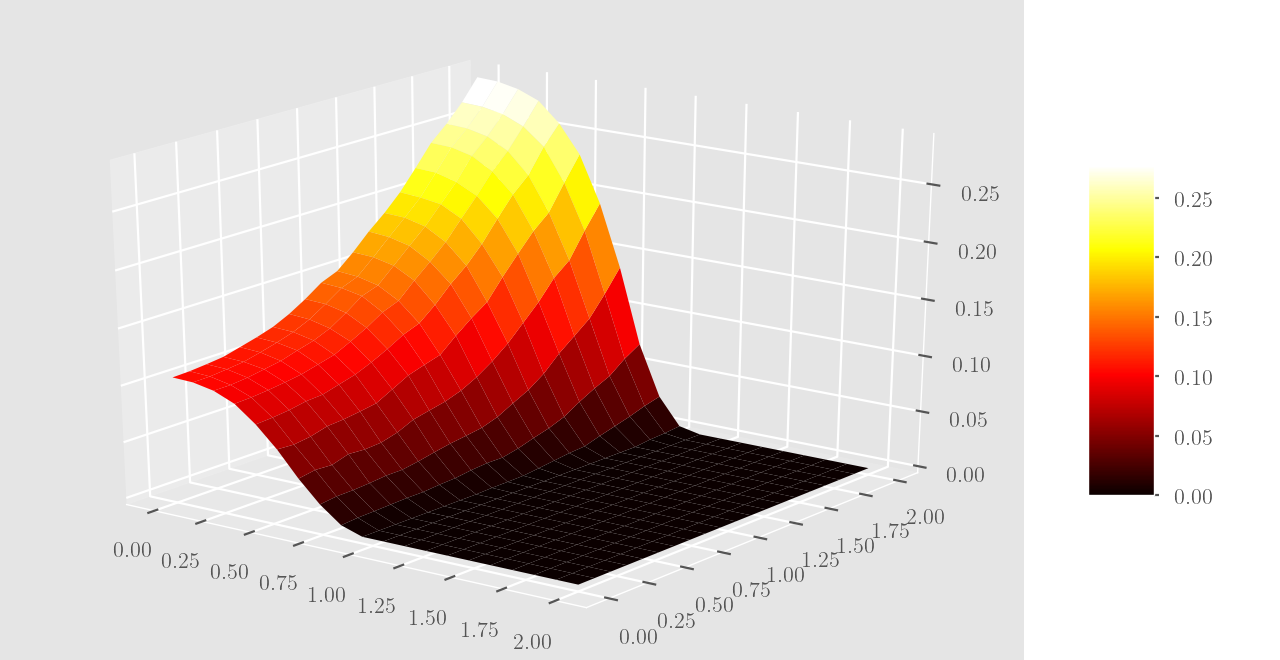
\includegraphics[scale=0.18]{figs/Figure_2} 
  \caption{$\beta$-DM}
\end{figure}
\end{multicols}
\end{frame}



%------------------------------------------------
\begin{frame}
\frametitle{Potential Energy}
\begin{equation}
\frac{\partial \Psi(\tilde{\mathbf{x}})}{\partial \tilde{\mathbf{x}}} \propto -\frac{\partial \log p(\tilde{\mathbf{x}})}{\partial \tilde{\mathbf{x}}} \cancel{\Rightarrow}\,  \Psi \propto -\log p
\end{equation}
\begin{multicols}{2}
\begin{figure}
\centering
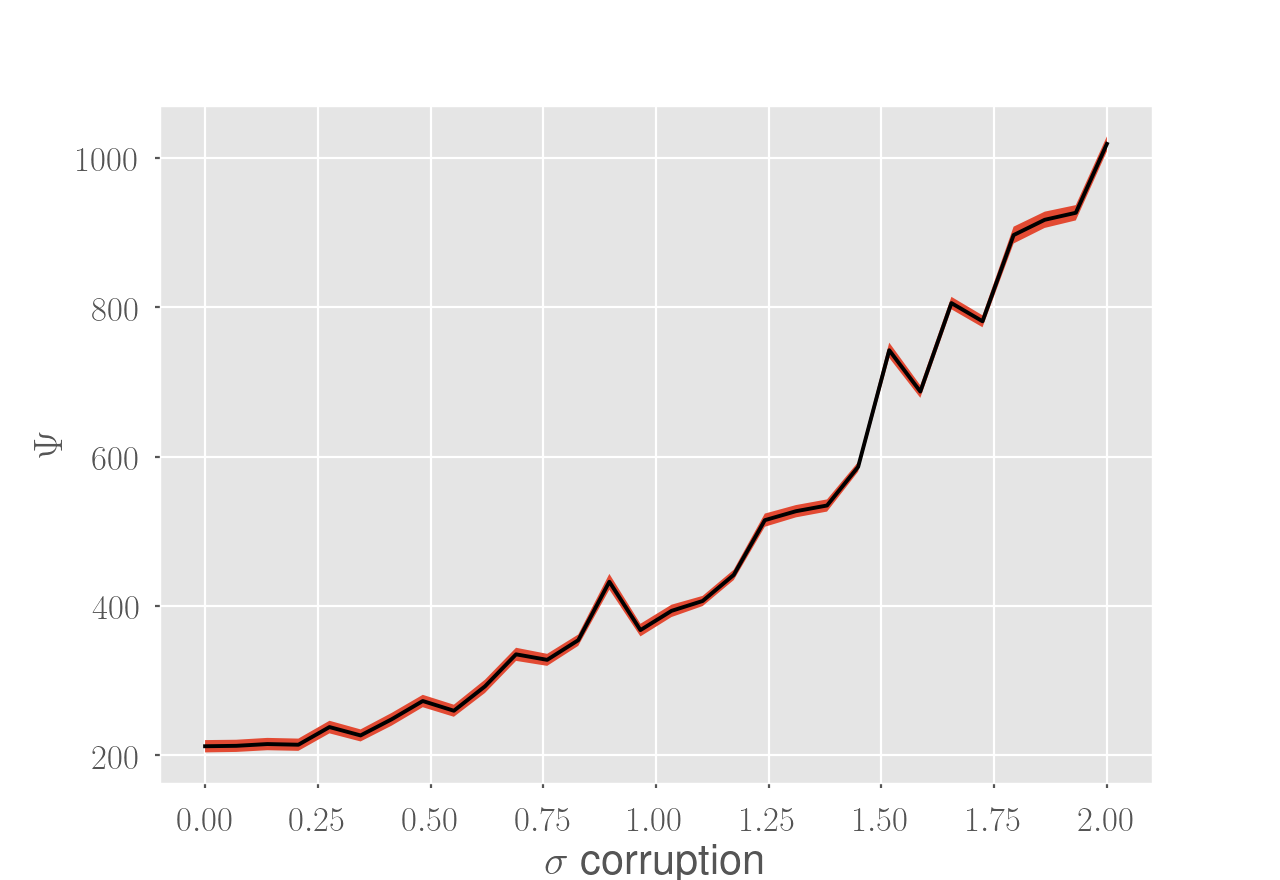
\includegraphics[scale=0.2]{figs/noisy-signal-dm-snr}
\caption{noisy DM-mode}
\end{figure}
\columnbreak
\begin{figure}
\centering
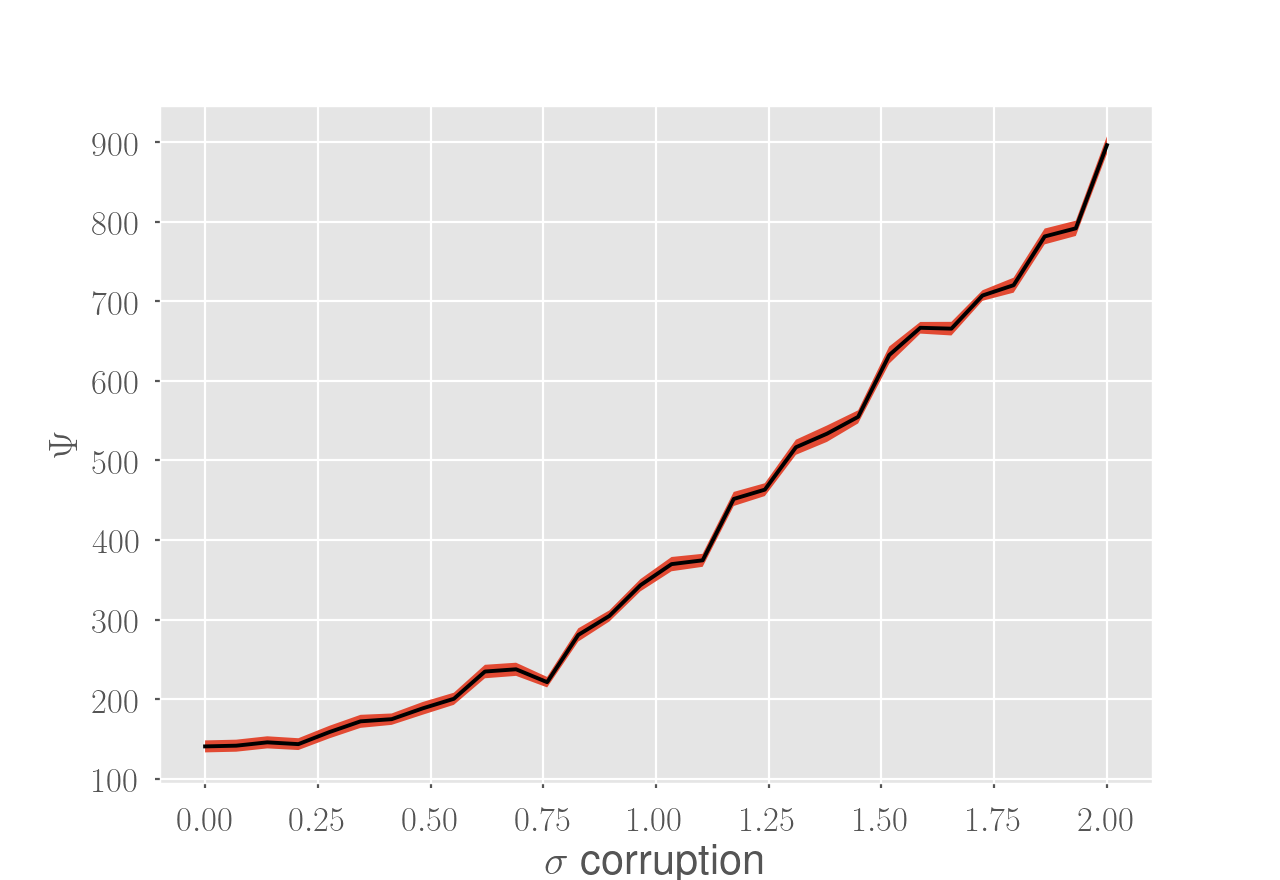
\includegraphics[scale=0.2]{figs/noisy-signal-ip}
\caption{noisy IP-mode}
\end{figure}
\end{multicols}
\end{frame}

%------------------------------------------------
\begin{frame}
\frametitle{Potential Energy}
\begin{multicols}{2}
\begin{figure}
\centering
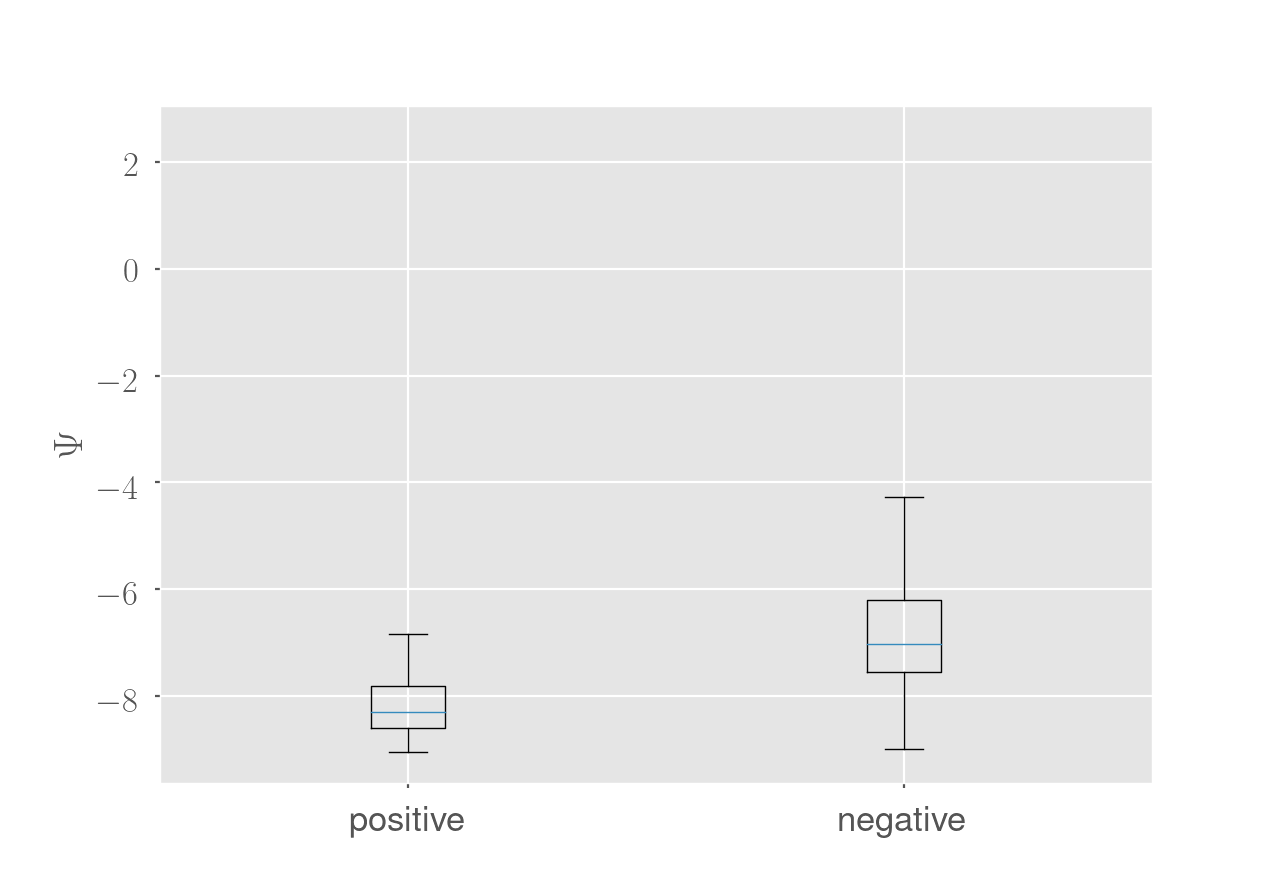
\includegraphics[scale=0.2]{figs/signal-vs-background-dm-snr}
\caption{DM-mode}
\end{figure}
\columnbreak
\begin{figure}
\centering
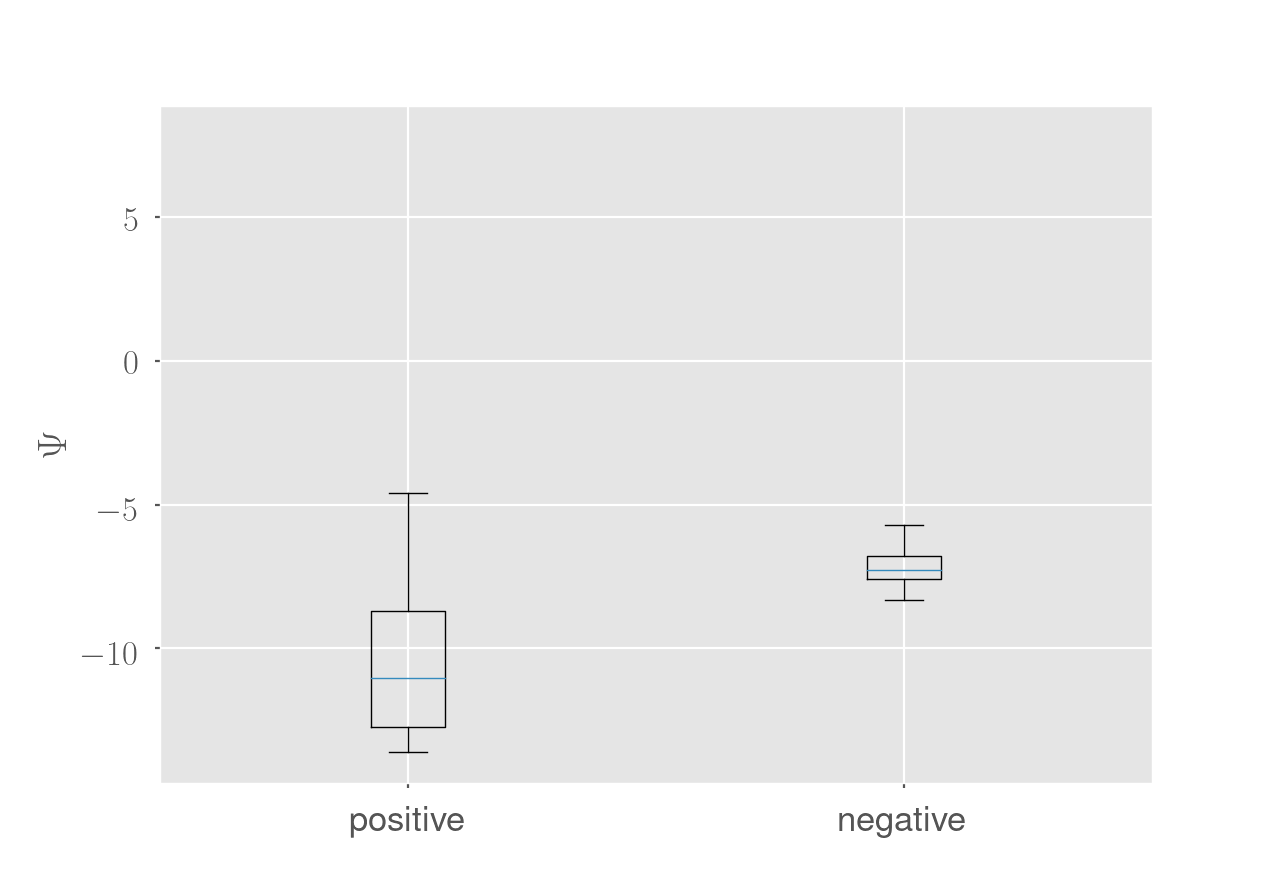
\includegraphics[scale=0.2]{figs/signal-vs-background-ip}
\caption{IP-mode}
\end{figure}
\end{multicols}
\end{frame}

%------------------------------------------------
\begin{frame}
\frametitle{F1-score?}
F1-score at NSR = 5 dB:\\[0.7cm]
\centering
\begin{tabular}{@{}rr|cc@{}}\toprule
groundtruth&noise & Correct & Wrong \\ \midrule\midrule
1 &normal & 0.9029 & 0.09701 \\
1 &IP-noisy &  0.6825 & 0.3174\\
1 &DM-noisy & 0.7297 & 0.2702\\\midrule
0 &normal & 0.9843 & 0.01563 \\
0 &IP-noisy &  0.8770 & 0.1229\\
0 &DM-noisy & 0.9503 & 0.04962\\
\end{tabular}
 \end{frame}
 

%------------------------------------------------
\begin{frame}
\frametitle{Alternative attention module}
\begin{multicols}{2}
\begin{figure}
\centering
\vspace*{1cm}
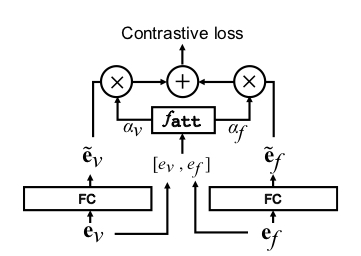
\includegraphics[scale=0.3]{figs/noise-tolerant-t}
\vspace*{0.82cm}
\caption{Model}
\end{figure}
\columnbreak
\begin{figure}
\centering
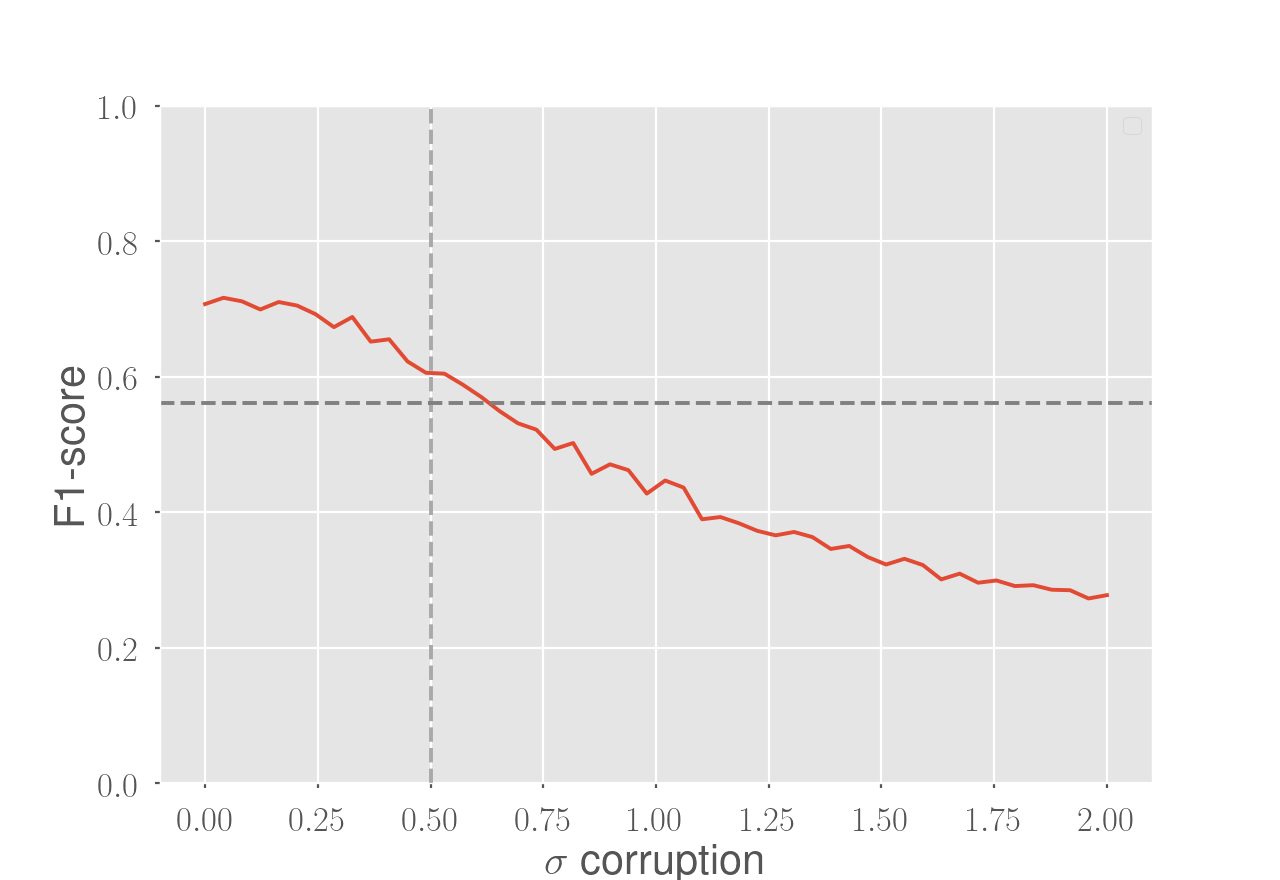
\includegraphics[scale=0.2]{figs/other}
\caption{F1-score}
\end{figure}
\end{multicols}
\end{frame}

%----------------------------------------------------------------------------------------

\end{document}
